\documentclass[11pt]{article}
\usepackage{upquote}
\usepackage{rotating}
\usepackage{alltt}
\usepackage{mathptmx}
\usepackage{helvet}
\usepackage{graphicx}
\usepackage[hmargin=1.3in,tmargin=1in,bmargin=1.5in]{geometry}
\usepackage{longtable}
\usepackage{url}
\usepackage[usenames,dvipsnames]{xcolor}
\usepackage{fancyvrb}
\usepackage{makeidx}
\usepackage[usenames,dvipsnames]{xcolor}
\usepackage{sectsty} % Allows to change section head style
\usepackage{tocloft}
\usepackage{hyperref}

\makeindex
\newcommand{\new}[1]{\index{#1}\emph{#1}}

\renewcommand{\cftsecpagefont}{ \sffamily\bfseries}
\renewcommand{\cftsecfont}{ \sffamily\bfseries}
\renewcommand{\cftsubsecpagefont}{ \sffamily}  
\renewcommand{\cftsubsecfont}{ \sffamily}  
\renewcommand{\cftsubsubsecpagefont}{ \sffamily}
\renewcommand{\cftsubsubsecfont}{ \sffamily}
\renewcommand{\contentsname}{}
\allsectionsfont{\sffamily\bfseries\color{NavyBlue}}

%\usepackage{draftwatermark}
%\SetWatermarkText{DRAFT}
%\SetWatermarkScale{1}

\definecolor{dark-almost-gray}{rgb}{0.2,0.2,0.4}

\hypersetup{
    colorlinks,
    citecolor=blue,
    filecolor=blue,
    linkcolor=blue,
    urlcolor=blue,
}

\makeatletter
\DefineVerbatimEnvironment{verbatim}{Verbatim}{xleftmargin=.25in}

\def\verbatim@processline{%
  \hspace{3in}\the\verbatim@line\par}
\renewcommand{\verbatim@font}{\ttfamily\small}


%\newcommand{\tag}[1]{$\texttt{<#1>}$}
\gdef\tagindexed{1}
\newcommand{\tag}[2][\relax]{%
  \ifcsname tagindexed#2\endcsname\relax\else%
  \index{#2@\texttt{$<$#2$>$}}%
  \expandafter\gdef\csname tagindexed#2\endcsname{\relax}\fi%
  \bgroup\tt$<$#2\ifx#1\relax\relax\else~#1\fi$>$\egroup}
\newcommand{\stoptag}[1]{\bgroup\tt$<$/#1$>$\egroup}
\newcommand{\startstoptag}[2][\relax]{\bgroup\tt$<$#2\ifx#1\relax\relax\else~#1\fi/$>$\egroup}
\newcommand{\element}[3][\relax]{\tag[#1]{#2}#3\stoptag{#2}}

\makeatother

\newcommand{\capt}[1]{\begin{minipage}{0.75\columnwidth}\itshape#1\end{minipage}}


\begin{document}

\title{Adding Computer Science Concepts to the Middle School
  Curriculum: A New Approach\thanks{Many thanks to NASA Space Grant
    and Dr.\,Peter Schultz for supporting this work.  Much gratitude
    is also owed to Dr.\,Chad Jenkins for initial guidance and
    inspiration.}}  \author{Tom Sgouros\footnote{Computer Science
    Department, Brown University, Providence RI,
    thomas\_sgouros@brown.edu}, Mike McGuigan\footnote{The Learning
    Community, Central Falls RI}} \date{21 September 2015}
\maketitle

\bgroup
\sffamily
\tableofcontents
\egroup

\setlength{\parskip}{\baselineskip}
\setlength{\parindent}{0pt}

\section{About this curriculum}

This curriculum was designed as a supplement to the ``tech readiness''
curriculum employed in many middle schools.  Most tech readiness curricula
treat the computer as a mere device to be used, a black box that runs
browsers, word processors, and spreadsheets.  But the computer is much
more than that: it is a tool that is shaping our future, and it is
also a tool that a user can shape.  The applications of tomorrow are
very likely going to bear only a passing resemblance to the ones in
use today.  Students should be equipped not only to operate today's
computer programs, but to understand computers well enough to operate
the programs of tomorrow.  And some students may create those
programs.  All students should be aware of that possibility.

This curriculum was developed at the Learning Community, a public
charter school in Central Falls, Rhode Island during the 2014--2015
academic year.  It was meant to be the first of three successive years
of lessons, with the second and third years looping through similar
material, adding more advanced concepts with each pass.

\subsection{Goals}
\index{goals!basic familiarity}

The goal of this curriculum is to provide basic familiarity with a
broad range of computer science concepts.  By the end of the
curriculum, students will be able to understand the components of a
simple computer program well enough to be able to modify it and
successfully change its function.  This will provide a base of
understanding for learning to design and write a program from scratch
in the future, though that is not a necessary part of this
curriculum.\footnote{As an aside, there are very few substantial
  computer programs that are actually ever created from scratch.
  Professional practice in the software industry is almost exclusively
  about modifying existing software, to accomplish new tasks or to
  eliminate bugs.  Even the simplest programs are typically copied and
  modified rather than starting from a blank page.}


\subsection{Method}
\index{methods!hands-on}

The twin components of practice for this curriculum are to take a
working computer program and learn to read it well enough to figure
out where to change it, and to engage in as much hands-on
experimentation as possible.  There will be some conceptual exercises,
included because they are both illustrative of important points, and
fun.

Lessons are meant to be accomplished in an hour-long class period,
beginning with a group discussion and moving to an exercise to be
tried by students.  Some of the lessons will involve a post-exercise
discussion and a few of them may be split among successive class
sessions.

\index{team learning}
The curriculum will require a computer for each student or student
team.  (Teams of two can be a highly effective method of learning this
material.)  No special software is required.  Because the necessary
software tools are readily available on any computer with a modern
browser program, such as Firefox, Safari, Chrome, or Internet
Explorer, we will focus on web programming, including HTML and
Javascript.  All modern web browsers contain some version of developer
tools to program with, and there are many web sites out there that
will support experimentation as well.

The curriculum does not use a simplified computer language, or a
language specialized for education, but uses simple examples in a real
and widely used language.

This curriculum makes heavy use of JSFiddle.net, a programmer's web
site, where students can test Javascript, HTML, and CSS stylesheets,
the essential pieces of programming for use on the web.  A school
system wanting to implement this curriculum at large scale might
consider duplicating that service on their own servers.

\subsection{Standards}
\index{CSTA standards}
\index{standards|see{CSTA standards}}
\index{curriculum standards}

This curriculum is aligned with the beginning of the level 2 defined
in the Computer Science Teachers Association (CSTA K-12 Computer
Science
Standards).\footnote{\url{http://csta.acm.org/Curriculum/sub/K12Standards.html}}
Upon completion of this curriculum, a student will have begun to
acquire the capacities described there and listed below.  The table
here indicates which of the CSTA standards are addressed in this
curriculum.  The CSTA page footnoted has links to tables describing the
alignment of the CSTA capacities with other widely-used curriculum
standards.

\begin{longtable}{lp{0.8\columnwidth}} \\
\multicolumn{2}{c}{CT: Computational Thinking} \\ \hline
CT.L2-01 & Use the basic steps in algorithmic problem-solving to design solutions (e.g., problem statement and exploration, examination of sample instances, design, implementing a solution, testing, evaluation). \\
CT.L2-03 & Define an algorithm as a sequence of instructions that can be processed by a computer. \\
CT.L2-04  & Evaluate ways that different algorithms may be used to solve the same problem. Act out searching and sorting algorithms. \\
CT.L2-05  & Describe and analyze a sequence of instructions being followed (e.g., describe a character’s behavior in a video game as driven by rules and algorithms). \\
CT.L2-06 & Represent data in a variety of ways including text, sounds, pictures, and numbers. \\
CT.L2-12  & Understand the notion of hierarchy and abstraction in computing, including high level languages, translation, instruction set, and logic circuits. \\
CT.L2-15  & Use predefined functions and parameters, classes and methods to divide a complex problem into simpler parts. \\ \hline

\multicolumn{2}{c}{\rule{0pt}{15pt}CL: Collaboration} \\ \hline

CL.L2-02 & Collaboratively design, develop, publish, and present products (e.g., videos, podcasts, websites) using technology resources that demonstrate and communicate curriculum concepts. \\
CL.L2-03 & Collaborate with peers, experts, and others using collaborative practices such as pair programming, working in project teams, and participating in group active learning activities. \\
CL.L2-04 & Exhibit dispositions necessary for collaboration: providing useful feedback, integrating feedback, understanding and accepting multiple perspectives, socialization. \\ \hline

\multicolumn{2}{c}{\rule{0pt}{15pt}CPP: Computing Practice and Programming} \\ \hline

CPP.L2-03 & Design, develop, publish, and present products (e.g., webpages, mobile applications, animations) using technology resources that demonstrate and communicate curriculum concepts. \\
CPP.L2-04 & Demonstrate an understanding of algorithms and their practical application. \\
CPP.L2-05 & Implement problem solutions using a programming language, including: looping behavior, conditional statements, logic, expressions, variables, and functions. \\
CPP.L2-06 & Demonstrate good practices in personal information security, using passwords, encryption, and secure transactions. \\
CPP.L2-07 & Identify interdisciplinary careers that are enhanced by computer science. \\
CPP.L2-08 & Demonstrate dispositions amenable to open-ended problem solving and programming (e.g., comfort with complexity, persistence, brainstorming, adaptability, patience, propensity to tinker, creativity, accepting challenge). \\\hline

\multicolumn{2}{c}{\rule{0pt}{15pt}CD: Computers and Communication Devices} \\ \hline


CD.L2-01 & Recognize that computers are devices that execute programs. \\
CD.L2-02 & Identify a variety of electronic devices that contain computational processors. \\
CD.L2-03 & Demonstrate an understanding of the relationship between hardware and software. \\
CD.L2-04 & Use developmentally appropriate, accurate terminology when communicating about technology. \\
CD.L2-08 & Describe ways in which computers use models of intelligent behavior (e.g., robot motion, speech and language understanding, and computer vision). \\ \hline

\end{longtable}


\subsection{Subjects --- Instructor background}

Some general information will be useful for the instructor to master.
This section provides a general background.


\subsubsection{Data}
\index{instructor background!data}
\index{data!instructor background}

\index{JPEG!as data}
\index{HTML!as data}
Data is a word widely used, but not widely understood.  Data is
information that \emph{means} something when used in a particular way.
A JPEG file is information that means an image, though it has to be
rendered in a particular way in order to be viewed.  A web page is
described by the data contained in an HTML file, style sheets, and
any incorporated scripts, and it has to be used in a particular way,
by a web browser.  A PDF file describes a document, usually a
printable one, and so on, for many different kinds of data.

There are many more forms of data than this.  Environmental data might
consist of a series of numeric measurements taken at specific times
and places.  Polling data is a collection of questions and records of
responses.  Modeling data is usually a suite of estimates describing
the state of the model at some time step.  Navigation data for a robot
might consist of the position and attitude of the robot, a map of the
room it's in, some words being spoken to it, and the camera view
ahead.  Some of this data is numeric and some is
alphabetic.\footnote{Though a computer stores both decimal numbers and
  alphabetic data as binary numbers, this is seldom anything more than
  an interesting digression for students who really want to know how
  it all works.  As interesting as it is, beginning programmers need
  not be troubled with the details of how data is actually stored and
  manipulated by a computer.}

There is an immense variety of data to consider.  Some forms of data
are highly regular.  Image file formats, for example are very
carefully described, even if the images they contain can vary
infinitely.  A program to handle that sort of well-described data will
be fairly different than another program to do statistical analysis on
some time series.

\index{vector!data}
\index{array!data}
\index{string!data}
Data values in a computer program can be singular, like a
number or a letter, or multiple, like a string of letters that make up
a word, or a collection of numbers.  Such a collection is called a
\emph{vector} or \emph{array} (if it's a collection of letters, it is
called a \emph{string}).  In addition, most modern computer
languages have a provision for more complicated collections of data,
such as the name and address of a student, plus his or her quarterly
grades, or all the pieces of a web page.  Many of the languages that
do not have such provisions have evolved conventions to substitute for
them.


\subsubsection{Variables}
\index{instructor background!variables}
\index{variables!instructor background}

An important concept in handling data is the \emph{variable}.  A
variable is simply a name linked to some value.  A variable called `j'
might refer to a number, as might another variable called `number'.
Another name, `student', might refer to a collection of data for Jack,
Sarah, Alisha, or Manuel.  With each of these, the first is the name,
the second is the value.  The name is arbitrary, and you could call a
number `j' or `henry' or `mike' or whatever you please.

\begin{center}
\includegraphics{variables.pdf}

\capt{A variable is just a name and a value.  Here are three names and
  three values.  The value of `student' is a complicated combination
  of other names and values but it's still one value.}
\end{center}

Most computer programs are written with variables, allowing them to
run on whatever data is appropriate.


\subsubsection{Programs}
\index{instructor background!programs}
\index{programs!instructor background}


A computer program is essentially a step-by-step recipe.  Step one do
this, step two do that, check and see if the result is good, do
something if it is, do something else if it is not.  The abstract
procedure is called an \new{algorithm}.  Some computer languages are
designed to make certain classes of algorithms simple, and some
languages contain exotic facilities for certain operations. For the
most part, you can create the same algorithm in any computer language;
the meaning is the same, even if the spelling and syntax might differ.

A program consists of operations, assignments, and control
structures.  An operation involves changing some piece of computer
memory with some arithmetic or logical function.  Adding two numbers
is an operation, as is subtracting, multiplying, taking the logical
complement, or some even more exotic calculation.  Assigning the
result of an operation to some variable allows a program to save it
for further operation or reporting to the user.

Control structures are used to change the order of operations and
assignments.  The three main categories of controls are conditionals,
loops, and calls.  A conditional checks some state---the value of one
or more variables---and uses that state to determine which parts of
the program to execute.  Here is a Javascript conditional that checks
the state of a variable x and sets a y variable accordingly:

\index{example!conditional}
\index{conditional!example}
\begin{verbatim}
if (x > 0) {
   y = 0;
} else {
   y = 1;
};
\end{verbatim}

If the variable x contains a value greater than zero, set the variable
y to equal zero, otherwise set y to one.

A loop is used to repeat some part of a program.  Some loops iterate
over a set of values, while others use a condition to control the
loop.  Here is a Javascript loop that executes an addition operation
five times while iterating over the members of a five-element vector.

\index{example!for loop}
\index{for loop!example}
\begin{verbatim}
y = 0;
for (x in [1, 2, 3, 4, 5]) {
   y = y + x;
};
\end{verbatim}

This loop will execute its \emph{body}, the statements betweeen the
curly brackets, once for each value of the [1, 2, 3, 4, 5] vector.
When finished, the variable y will contain the value 15.

A \emph{call} is the last of the important control structure
categories.  This is a way to break up a program into sub-programs,
called \emph{functions} or \emph{subroutines}.  This does not change
their function, but it makes it easier to understand a big program and
split it up into understandable pieces.  Here is a Javascript function
that accepts two numbers and returns their sum:

\index{example!function}
\index{function!example}
\begin{verbatim}
add = function(x, y) {
  return( x + y );
};
\end{verbatim}

A program that uses this function will have statements in it that look
like this:

\begin{verbatim}
add(7, 5)
add(p, q)
\end{verbatim}

This can make code easier for a person to read.  This may not seem
like an important feature, but maintaining a complicated program
across generations of operating system changes and demands for new
features will always require frequent rewrites.  Code that is readily
understood can be readily updated.  Unreadable code can seldom be
updated, or if updated has a high risk of introducing errors.

The other great value of a function is that it provides for the
creation of function \emph{libraries}, collections of functions that
can be distributed as the building blocks of a complex program.  For
example, a library might contain advanced math calculations, or
graphics instructions.  Depending on the language, these are also
sometimes called \emph{packages}.

Of course functions, loops, and conditionals can be tremendously more
complex than these simple examples, but the principles are exactly the
same as these simple examples.


\section{Unit 1 -- Computer Programming}

Computers rule our world.  They are present not just in the screens
and keyboards of desktops and laptops, but also in cars, toasters,
phones, robots, cameras, and stoves.  Computers not only use
electricity, but also make it possible to have a functioning grid of
wires to bring electricity to your house.  The transportation network,
including trains, planes, boats, and cars, all depend on computers.
The financial network of banks, brokers, investment funds, and
insurance companies do, too.


\subsection{What is it?}

Writing a computer program is like writing a cookbook recipe for an
idiot.  Computers today can do amazing things, and they do them very
quickly, so we mistake them for ``smart.''  In fact, from a
programmer's perspective, the computers of 2015 are very stupid, and
only do exactly what they are told and only know what we tell them.
Even the fanciest robot, the most impressive trivia-competing or
chess-playing program, has only a hazy ``idea'' of the world we
inhabit, and there are no computer programs that can carry on a
conversation and \emph{mean} what they say, even if there are
computers that can react appropriately to most voice commands you give
them.

\subsubsection{Discussion: What is programming?}

The way to begin a discussion about programs is with examples of
recipes.  Here is a recipe for pancakes:

\begin{enumerate}
\item Beat one egg, add one cup of milk and two tablespoons of oil.

\item Add one cup flour, two teaspoons baking powder, mix gently.

\item Heat griddle until a drop of water thrown on it sizzles.

\item Pour pancake batter onto the griddle, wait until bubbles form
  and pop, turn, count to thirty in your head.

\item Remove and eat.
\end{enumerate}

But cookbook recipes are not the only ones out there.  Who else has a
recipe for doing things?  What's your recipe for:

\begin{itemize}
\item Getting to school in the morning.

\item Doing homework.

\item Finding somewhere to sit at lunch or in a classroom.

\item Braiding hair or painting nails.
\end{itemize}

For several of these, the most important steps are the steps involving
making a decision.  These are places where you have to gather
information from the world, compare it to rules in your head, and come
out with a decision about what to do.  In the pancake example, the
most important step is deciding when they're done, and in the homework
recipe or the braiding recipe, probably the most important step is
deciding when to sit down and do it.  In the exercise, we'll imagine a
robot trying to make a decision about something important.


\subsubsection{Exercise: What is programming?}

Imagine a rolling robot wandering around a classroom.  It
has a camera to look at different objects in the room.  Make up a
recipe (an \emph{algorithm}) to decide whether some object is suitable
for a person to sit on.  Remember, it won't know the words for
``chair'' or ``leg'' (of a chair) or ``back'' (of a chair), or even
``sit'', unless you define them for it.

Students split up into groups of two or three to prepare a recipe for
deciding about some object.  A paper with step numbers on it will help
to arrange the recipe into distinct steps, something that is necessary
for a computer.  Reconvene the group and discuss the attempts together
with a couple of example chairs and other classroom objects to look at
in the middle.  Nominate one student to be the robot, examining and
judging objects, while the teacher leads discussion by reading the
instructions and watching the student follow them literally.

\begin{center}
\begin{tabular}{|l|p{3in}} \hline
1. & {\tt Does it have a flat spot?} \\ \hline
2. & {\tt If there is a flat spot, is it clean?} \\ \hline
3. & {\tt Is it tall enough?}\\
\end{tabular}
\end{center}

Background: Many classrooms will have four-legged classroom chairs.
Many will also have desk chairs on wheels, or stools.  Students also
have backs and legs; are they good for sitting on?  A hamster has four
legs and a back.  Is a table a good thing to sit on?  How about the
floor?  A chair is a good thing to sit on, but how about a broken
chair?  A stacked chair?  What about a chair with a book on it?  Or a
chair with a thumbtack on the seat?

Classification problems like these are open questions in computer
science.  That is, in 2015, there does not exist a robot in the world
that can identify all the different kinds of chairs in the world as
reliably as any average kindergarten student.

\subsection{More discussion: What do programmers do?}

The field of computer science is a rich one.  There are a lot of
problems out there to work on, many of which have no well-known
solution.  Understanding what are the range of topics people work on
is part of equipping students to understand the world ahead of them.
Here is a very incomplete list of the kinds of things computer
programmers are working on these days.

\begin{description}

\item[Graphics and visualization] There is a great deal of research
  ongoing about how people understand visual images, and how that can
  be harnessed to help us understand complex phenomena.

\item[User experience] Making a computer easy to use is something
  that few would call a ``solved'' problem.

\item[Performance design] The best possible way to design and run a
  computer has not yet been discovered.  There is a lot of work
  ongoing, in both hardware and software, to make computers run faster
  and the machines smaller.

\item[Databases] As it becomes apparent how useful data can be, more
  of it gets collected, for better and sometimes worse.  Understanding
  and solving the problem of storage and retrieval in giant databases
  becomes more and more important as they grow.  A database with a
  million entries is not useful if it takes a thousand times longer to
  search than a database with a thousand entries.

\item[Data science] Now that we have so much data about everything,
  analyzing it in useful and interesting ways has become a field of
  its own.

\item[Web design] This is an amalgam of many of the other pieces ---
  graphics, user experience, databases, even language --- but in the
  market, it is pretty much its own thing.  There is no perfect web
  site, so people and companies who need web sites will continue to
  look for new solutions.

\item[Control] There are a lot of seemingly controllable systems out
  there that are widely considered to be good candidates for
  automation, but also a lot of such systems that don't work
  very well.  Controls for electrical grid, or commodities
  markets, are two examples of systems in daily use that desperately
  need improvements for speed and reliability.

\item[Mapping] How to optimize travel and mapping seems like a solved
  problem, but it is far from that, even if computers can routinely
  turn out travel directions that seem fairly good.

\item[Robotics] Controlling a robot to move around and do useful work
  in the real world.  There are lots of robots that are almost useful,
  but there is a large gulf between ``almost'' and ``useful.''  If
  robots were useful and safe, you would see many more of them around.

\item[Human language] Getting a computer to understand human language
  in a useful way reamins an unsolved problem.  There are computer
  translators that work, but none that work well.

\end{description}

Beyond all this, there are many areas that are very difficult to
predict.  Quantum computing, virtual reality, wearable electronics,
low-energy computing---and who knows what else?---will shape our
future, but we don't know which parts will do it first.  The future
will belong to the software designers and inventors who figure it out.


\section{Unit 2 -- Data}

In its rawest form, all data in a computer is simply binary numbers.
To be useful or interesting, those numbers must relate to something in
the world.  The way the numbers relate to the world is defined by a
person.  For example, binary numbers can be used to model decimal
arithmetic, much more useful than binary arithmetic.  This is a
challenge engineers have met and mastered, but there are many more.
Encoding an alphabet---choosing which numbers represent which
letters---is another such problem, and one that has recently changed
dramatically, to incorporate non-latin alphabets.  It's not clear that
there won't be further important revisions to that encoding, and there
are many more that await a widely-used solution.  For example, say
you're building a robot to move around a room, how do you encode the
map of the room when all you have to use is numbers?  How do you
encode a map of the state?  A picture of a frog?  A hit song?


\subsection{Image data}

Modeling image data is an area where many students will have already
had some exposure to the problem.  The GIF, PNG, and JPEG formats are
widely used, but for different purposes.

\subsubsection{Discussion: How to describe an image}

A picture is a picture, but how do you make it into information a
computer can operate on?  The image itself is not something that can
be stored or operated on.  This is as true for a brain as for a
computer.  You can remember images, but no one thinks there is a stack
of photographs in between your ears.  The way a computer stores or
sends an image is by creating a description of that image and storing
that.

\subsubsection{Exercise: Describe an image}

Students split up into pairs, arranged into two long lines, back to
back.  One side receives a secret image to describe, while the other
side has a blank piece of paper and a pencil.  The task is for the
students with the image to describe the image to their partners, while
the partners draw it.

\begin{center}
\includegraphics[width=0.35\columnwidth]{pix-for-presentation/IMG_0494.jpg}~\includegraphics[width=0.62\columnwidth]{pix-for-presentation/IMG_0495.jpg}
\end{center}

Giving each side a ruler to draw with might help make things more
precise, and the teacher can model some ways to accomplish the task,
for example showing that the drawing is made from lines that can be
measured and located.  The drawing should be a relatively simple one,
with only a few elements.

After students have had a chance to make a drawing, switch the
exercise by giving the other side a different drawing, and reversing
the roles.  This time, the original drawing is superimposed on graph
paper, and the students tasked with reproducing it have graph paper to
draw on.  Does the strategy differ for getting a good reproduction?

\subsubsection{Post-exercise discussion}

Gather in the middle to look at the drawings, to discuss.  What made
reproducing the drawing easy or hard?  Were the descriptions precise
enough to be useful?  Some examples of student work are below.

\begin{center}
\includegraphics[width=0.2\columnwidth]{pix-for-presentation/snowman-orig.png}
\includegraphics[width=0.25\columnwidth]{pix-for-presentation/snowman-1.png}
\includegraphics[width=0.25\columnwidth]{pix-for-presentation/snowman-2.png}
\includegraphics[width=0.25\columnwidth]{pix-for-presentation/snowman-3.png}
\includegraphics[width=0.25\columnwidth]{pix-for-presentation/snowman-4.png}
\includegraphics[width=0.25\columnwidth]{pix-for-presentation/snowman-5.png}
\includegraphics[width=0.25\columnwidth]{pix-for-presentation/snowman-6.png}

\capt{The original drawing and several renditions.}
\end{center}

There are two major groups of graphical image storage formats: vector
and raster.  Vector graphics keep track of the position and location
of each line that makes up a drawing, while raster graphics keep track
of each dot.  Vector graphic formats, like PostScript, PDF, and SVG,
are best for line art and graphic elements, like fonts and graphs.  A
vector graphic can be reproduced at any scale without loss of
resolution.

Raster graphic formats, by contrast, do not keep track of the lines
themselves, but of which cell of a grid those lines cross.  To make a
raster image, the computer splits the image up into little cells and
records the color of each cell.  Raster formats include GIF, PNG, and
BMP, among others.  Raster images are sensitive to the scale.  That
is, if you blow up the image, you can see the pixelation of the lines
in the image.

This means that some images are more suited to one kind of image
format or the other.  In general, raster formats are better for images
with many gradations of colors and less sharp edges, while vector
formats are better for images with fewer colors and sharp edges.
Fonts for printing, for example, are usually stored as a vector
format, while photographs are usually better rendered in one of the
raster formats.  The next two pages contain examples of images better
rendered as one or the other, shown as both, and enlarged considerably
so you can see the differences easily.  At a normal scale, of course,
the differences would be more difficult to see.

\newpage
\thispagestyle{empty}
\begin{sideways}
\begin{minipage}{8.5in}
\begin{center}
VECTOR \hspace{4in} RASTER

\vspace{0.9in}
\includegraphics[width=4in]{dopey.pdf}
\includegraphics[width=4in]{dopey.png}
\end{center}
\end{minipage}
\end{sideways}
\newpage
\thispagestyle{empty}
\begin{sideways}
\begin{minipage}{8.5in}
\begin{center}
VECTOR \hspace{4in} RASTER

\vspace{0.9in}
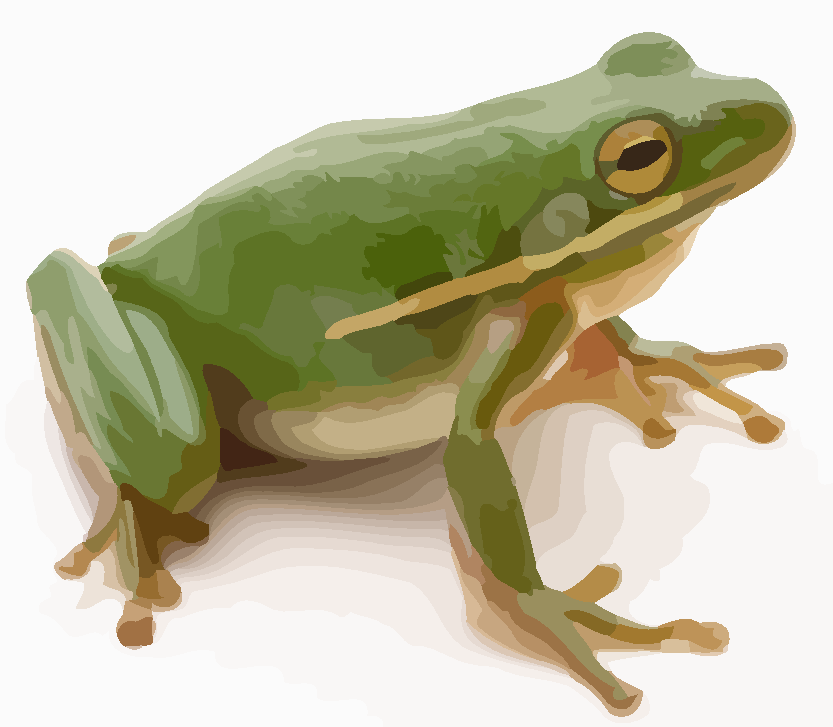
\includegraphics[width=4in]{frog.pdf}
\includegraphics[width=4in]{frog-reduced.jpg}
\end{center}
\end{minipage}
\end{sideways}
\newpage

\subsubsection{Discussion: Raster Images}

Another potential exercise involves demonstrating how raster images
work.  For a raster image, you divide the scene up into a grid, and
measure the color and intensity of each square of the grid.  The hope
is that the grid squares are small enough that the viewer doesn't
really notice them.  On a screen, there are usually 75-100 dots per
inch, and quality printed material is often greater than several
hundred dots per inch.

\subsubsection{Exercise: Raster images}

Give teams of students a raster image in disguise and have them color
it in as a team, to show how you can make an image out of a big grid
of numbers.  See the following page for an example.  This page could
be handed out to the teams as is.

For the exercise on the following page, you'll need a way to apply
colors to a board.  Students will need four colors, preferably in some
sort of graded series, like white, light green, dark green, black.
This could be coloring squares on a large paper, or applying colored
sticky notes.  Sticky notes, being square, will be fairly easy to
apply in straight lines.

(If you can only find three color grades, the two middle grades can be
combined and the results will still be acceptable.)

\newpage
\thispagestyle{empty}

Each team has four different colors to use. Put colors on the board
according to the table, in the row corresponding to your team's
number.

\newcommand{\propmeup}{\raisebox{-9pt}{\rule{0pt}{25pt}}}

\begin{center}
\raisebox{1in}{\begin{sideways}
If the number in the table is:
\begin{tabular}{ll}
less than 10 & use color 1 \\
10 or greater and less than 100 & use color 2 \\
100 or greater and less than 200 & use color 3 \\
200 or greater &  use color 4 \\
\end{tabular}
\end{sideways}}
\hspace{25pt}
\begin{sideways}
\begin{tabular}{l|ccccccccccccccc}
\propmeup Team 1 & 0 & 8 & 254 & 251 & 255 & 254 & 254 & 255 & 255 & 81 & 3 & 1 & 82 & 255 & 255 \\ \hline
\propmeup Team 2 & 7 & 7 & 255 & 255 & 249 & 255 & 255 & 167 & 0 & 4 & 82 & 173 & 0 & 2 & 252 \\ \hline
\propmeup Team 3 & 0 & 8 & 255 & 255 & 255 & 247 & 252 & 86 & 0 & 169 & 255 & 251 & 168 & 1 & 172 \\ \hline
\propmeup Team 4 & 0 & 8 & 255 & 250 & 253 & 255 & 255 & 2 & 0 & 255 & 251 & 255 & 255 & 168 & 255 \\ \hline
\propmeup Team 5 & 1 & 8 & 255 & 255 & 255 & 254 & 247 & 0 & 86 & 255 & 255 & 255 & 250 & 255 & 255 \\ \hline
\propmeup Team 6 & 0 & 8 & 250 & 255 & 254 & 255 & 255 & 1 & 90 & 251 & 250 & 254 & 255 & 254 & 251 \\ \hline
\propmeup Team 7 & 0 & 8 & 255 & 253 & 255 & 250 & 255 & 81 & 0 & 255 & 255 & 255 & 167 & 5 & 170 \\ \hline
\propmeup Team 8 & 0 & 3 & 1 & 3 & 3 & 1 & 254 & 173 & 1 & 0 & 84 & 86 & 0 & 0 & 255 \\ \hline
\propmeup Team 9 & 0 & 0 & 1 & 0 & 0 & 0 & 255 & 255 & 170 & 85 & 0 & 0 & 85 & 169 & 255 \\ \hline

\end{tabular}
\end{sideways}
\end{center}
\newpage

% \subsection{Images and compression (Advanced)}

% Image formats (and video) are their own fun topic because they have to
% be compressed to be useful, and compression is an interesting topic to
% play with, and can be done with instruction/reconstruction exercises
% that might be fun.




\subsection{Web pages}

Like a graphical image, a web page is transmitted as a description of
that page, in a well-defined format called HTML.  HTML marks which
parts of a document are headings, which are text, where images are to
be placed, and more.  Additional information indicates the color and
style of the text, and other features.

\index{HTML!open and close tags}
\index{element!open and close}
\index{tag!HTML}
HTML is formatted as text surrounded by ``open'' and ``close'' tags.
An open tag looks like this: \tag{p} while a close tag looks like
this: \stoptag{p}.  If a \tag{b} implies a bold face, the
following puts a serene calmness in bold:

\index{example!bold font}
\index{ataraxy}
\begin{verbatim}
<b>ataraxy</b>
\end{verbatim}

There are paragraph-level HTML tags, for headings, paragraphs, lists,
quotations, and more, and character-level HTML for bold, italic,
underlines, and so on.  You can also have single-tag HTML elements,
that look like this:

\index{example!single-tag element}
\begin{verbatim}
<br/> or <hr/>
\end{verbatim}

\index{HTML!break}
\index{break!HTML}
\index{horizontal line!HTML}
\index{line!HTML}
These elements put a break in a page and a horizontal line,
respectively.  Other elements that are commonly seen as single tags
are image tags (\tag{img}) and canvas (\tag{canvas}) about which we'll
hear much more in section~\ref{canvas}.

An element can also contain \new{attributes}, values that modify the
element in some way.  To change the size of a font, for example, you
could include a ``size'' attribute to a ``font'' tag:

\index{example!font size}
\begin{verbatim}
Regular text <font size="+1">bigger text</font> regular text.
\end{verbatim}

One of the most important things about HTML elements is that they can
contain other elements.  An \tag{html} element will contain a
\tag{body} tag which can contain multiple \tag{p} elements, and those
\tag{p} elements can contain multiple \tag{font} changes and other
elements and so on. (And on and on.)


In the example below, the \tag{body} element contains two \tag{p}
elements.  The first of them contains some text, some of which is
itself inside an \tag{i} element (indicating italics) and an
unordered list (\tag{ul}) with two list items (\tag{li}).  The second
\tag{p} element contains only text.

\index{example!HTML page}
\index{HTML page!example}
\begin{center}
\label{htmlfig}
\begin{minipage}{0.5\columnwidth}
\begin{verbatim}
<body>
  <p><i>Fall</i> is the time for:
    <ul>
      <li>Falling leaves</li>
      <li>Back to school</li>
    </ul>
  </p>
  <p>And more!</p>
</body>
\end{verbatim}
\end{minipage}
\begin{minipage}{0.49\columnwidth}
\begin{center}
\includegraphics{fall-is.pdf}
\end{center}
\end{minipage}

\capt{A web page and the structure of the web page.  It looks like
  this in a browser:} 

\includegraphics[width=0.67\columnwidth]{fall-is.png}
\end{center}


As you might imagine, this explanation just scratches the surface, and
this kind of page structure can become absurdly complex.  (And \tag{i}
elements are obsolete, too.  We use \tag{span} and stylesheets now.)
But however complex the page, the basic elements function in this same
basic way.

When you're talking about dynamic web pages (which is what you're
talking about when you're talking about Javascript), the web page in
which a program runs is among the more important pieces of data to be
operated on, and even has its own special name, the \new{document}.
Dynamic pages read from, and modify, the web page they're embedded in,
so understanding what they are and how the hierarchy of HTML works is
a key part of making them work.

\subsubsection{Discussion: Look at a web page under the covers}

HTML is what all web pages look like inside, no matter how
complicated.  For a complicated web page, it can be challenging to see
the HTML, but it is there.  There are some simple web pages out there
to find and show to students.  Try to find some without a lot of
scripting and style sheets, and use the ``View Source'' option on your
browser to see the HTML underlying the page.\footnote{This is in a
  different place on each brownser, but it is there in all of them.
  Look under ``Developer Tools'' if that option exists, or ``View.''}

Wikipedia has fairly simple pages, for example.  Show the class a
side-by-side comparison, and point out the tags that make up the page
for some random choice of web site.  Modern web sites are complex
affairs, but the HTML tags can be seen there.


\subsubsection{Exercise: Make a web page}

Students go open JSFiddle accounts, if they do not have them already.
The teacher should keep track of student account names \underline{and
  passwords}.\footnote{JSFiddle claims to require an email in order to
  open an account.  This is not true, you can enter a fake email
  account, but you will have no recourse if you lose the password.
  But there is no security risk here---there need be no personal
  data entered---so easy passwords are fine.}

To start a project, click on ``New project'' or ``Editor,'' and type
this in the HTML (upper left) pane of the window:

\begin{verbatim}
<h1>My name</h1>
<p>My name is Bftsplk</p>
\end{verbatim}

Click on ``Run'' and the rendered web page will appear in the bottom
right pane.


This is not very exciting, and typing is slow.  The teacher should
prepare a JSFiddle with a simple web page with a few paragraphs and
headings, like this:

\index{example!HTML page}
\index{HTML page!example}
\index{example!web page}
\index{web page!example}
\begin{verbatim}
<body>
<h1>How HTML works</h1>
<h2>Elements</h2>
<p>HTML is what is called a "markup language" which means that the
text and the instructions about how to format the text are mixed
together. HTML is a particular version of a family of languages called
"SGML". You may have heard of XML which is the other popular SGML.
These languages all look similar with "elements" marked with "start"
tags (that look like &lt;tag&gt;) and "close" tags (that look like
&lt;/tag&gt;).</p>
<hr/>
<p>HTML elements often contain other HTML elements, so a paragraph
element might contain:
    <ul>
        <li>A list;</li>
        <li>Some <em>emphasized</em> text;</li>
        <li>Some <code>code</code>.</li>
    </ul>
</p>
<p>If we say that an element that contains another element is its
parent, you can draw a kind of family "tree" for a page of HTML.</p>
<br/>
<p>You can edit this page by typing in the upper left window. Click on
"Run" up at the top to see what you changed. Can you add a paragraph?
How about adding an item in the list just above here? Then maybe add a
header up at the top with the &lt;h1&gt; tag using your name, followed
by a &lt;p&gt; element describing yourself?</p>
<h2>Functional Structure</h2>
<p>HTML was designed to describe the functional structure of a page of
text, not the way it looks. The markup for this paragraph, for
example, just says "p" for "paragraph". The list above is labeled "ul"
for "unordered list". The browser that displays the paragraph or the
list decides how it looks.</p>
</body>
\end{verbatim}

The teacher can just copy and paste from this document into his or her
own fiddle.

\index{JSFiddle!clone page}
\index{clone page!JSFiddle}
Students can ``clone'' this web page by:

\begin{itemize}
\item Log in to their own JSFiddle account.

\index{simplifying URLs}
\item Go to the URL of the example web page.\footnote{JSFiddle uses
    ``hashes,'' strings of random characters to identify projects.
    When JSFiddle was first created, the hashes were only two or three
    characters long, so easy to remember.  As JSFiddle became more
    popular, the hashes had to grow longer and are now quite
    unwieldy.  You can simplify the URLs for students with tinyurl.com
    or bit.ly or some similar URL-shortening service, some of which
    allow the teacher to choose a string to use.  So you could tell
    students to go to ``tinyurl.com/lc-lesson3'' for example, and
    students will be redirected to the teacher's fiddle.}
\item Click ``clone''.  Students will see the teacher's account name
  disappear from the URL and be replaced with the student's account
  name.
\end{itemize}

The assignment is simply to edit the HTML, to change it from what it
is to another subject, maybe about food they like?  Find and change
the color of the background and the font.

\index{save your work!JSFiddle}
\index{update!JSFiddle}
\index{JSFiddle!save}
\index{JSFiddle!update}
\index{JSFiddle!base}
\index{base!JSFiddle}
IMPORTANT: Use the ``Update'' button to save your work. JSFiddle will
save work with version numbers appended to it.  Use the ``Set as
base'' button to make the latest version be the one that appears
without the version number.

\begin{center}\setlength\fboxsep{13pt}
\framebox{\begin{minipage}{0.8\columnwidth}Most of the discussions and exercises that follow will proceed this
way, with a prepared web page students can clone into their accounts
and then edit to achieve some goal.
\end{minipage}}
\end{center}

\newpage
\thispagestyle{empty}
\subsubsection{HTML Elements}

There are dozens of different HTML elements available. Here are some
students can play around with.  Try putting these into the web page
and seeing what happens.

\begin{tabular}{ll}\\

\multicolumn{2}{c}{\bf These elements format a block of text.} \\
&\\
paragraph        & \element{p}{text here} \\
top-level heading& \element{h1}{heading} \\
2d-level heading & \element{h2}{heading} \\
3d-level heading & \element{h3}{heading} \\
formatted text   & \element{pre}{text~that~~keeps\,its~~~~spacing} \\

&\\

unordered list   & \element{ul}{\element{li}{item1}\element{li}{item2}} \\
unordered list   & \element[type="circle"]{ul}{\element{li}{item1}\element{li}{item2}} \\
ordered list     & \element{ol}{\element{li}{item1}\element{li}{item2}} \\
ordered list     & \element[type="A"]{ol}{\element{li}{item1}\element{li}{item2}} \\
ordered list     & \element[type="I"]{ol}{\element{li}{item1}\element{li}{item2}} \\

&\\

\multicolumn{2}{c}{\bf These elements format text inside a block.} \\
&\\
bold             & \element{strong}{bold text} \\
emphasis (italic)& \element{em}{italic text} \\
typewriter       & \element{code}{code text} \\
blink            & \element{blink}{very irritating blinking text} \\

change color     & \element[color="yellow"]{font}{red text} \\
change size      & \element[size="+2"]{font}{big text} \\

&\\
\multicolumn{2}{c}{\bf Another way to change text.} \\

&\\

change color     &  \element[style="color:~red;"]{p}{red text} \\
change font      &  \element[style="font-style:~italic;"]{h2}{italic text} \\
change size      &  \element[style="font-size:~200\%;"]{li}{big text} \\

\end{tabular}

Also try giving the \tag{body} tag a \texttt{bgColor="red"} or
\texttt{font="blue"} or (worse) both.


\newpage
\subsection{Including other information}

One of the real powers of the world-wide web is that any web page can
include a reference to other web pages.  This might be through a link,
but content can be included as well.  For example, an image is
included in a web page by reference to its URL.  Any modern web page
contains dozens or hundreds of such references.

\index{URL!definition}
\index{Uniform Resource Locator|see{URL}}
What is a URL?  A ``Uniform Resource Locator'', this is the familiar
string that you type into the navigation bar of your browser:

\index{URL!example}
\index{example!URL}
\begin{verbatim}
http://fancyserver.com/subject/file
\end{verbatim}

\index{http!URL protocol}
This string identifies a server, an optional subject category, and a
specific file.  The ``http'' specifies the kind of message that will
contain the requested information.  Other protocols are available, but
few users will see them often.

The ``file'' part of the URL can refer to a file containing HTML, but it
could also refer to an image or other kinds of information like a
stylesheet, or a collection of Javascript functions.  For now, let's
look at images and links.

\subsubsection{Discussion: External references}

\index{images}
There are two important types of external reference: images and links.

An image tag looks like this:

\index{example!image tag (img)}
\begin{verbatim}
<img src="http://imageserver.com/funnyimage.jpg"/>
\end{verbatim}

This instructs your browser to save some space on the web page it is
showing you, and fill that space with the image at the given URL.

The \tag{img} element supports a ``width'' attribute,
so you can squeeze a big image into the small JSFiddle window:

\begin{verbatim}
<img src="http://imageserver.com/funnyimage.jpg" width="250"/>
\end{verbatim}

\index{link}
Another common external reference is a link, the highlighted words you
click on to send your browser to another web site.  A link uses the
\tag{a} element, and looks like this:

\index{link!example}
\index{example!link}
\begin{verbatim}
<a href="http://newserver.com/newlink.html">linked text</a>
\end{verbatim}



\subsubsection{Exercise: Include external references}

Students should log into JSFiddle, where they should find the fiddle
from the previous class.

Students should find some images on the internet, and use \tag{img}
elements to incorporate them into their web page somewhere.

Then find another web page and create a link to that page in their
JSFiddle page.  Wikipedia has several pages to explain this or that
HTML element, so those would be good choices for a page about HTML.

\subsection{Stylesheets}

\index{Cascading Style Sheet|see{CSS}}
\index{CSS}
\index{stylesheet|see{CSS}}
Modern web pages very seldom use element attributes to control colors
and fonts and so forth.  Instead, they use ``Cascading Style Sheets''
(CSS) to control these aspects of a page, leaving the HTML to describe
structure alone.  In fact, the ``bgColor'' and ``text'' attributes
of the \tag{body} element are no longer supported in HTML5.  (Most
browsers will continue to draw them, though.)

\subsubsection{Discussion: How to control a page's style}

In order to control a page's elements, you have to be able to refer to
them, and then you have to be able to describe what is to be done.  A
CSS is made up of pairs of information, the first part of which
identifies which elements the second part is to affect.

\index{CSS!turn elements red}
For example, this bit of CSS will turn all the \tag{p} elements red:

\index{example!CSS}
\index{CSS!example}
\begin{verbatim}
p {color: red;}
\end{verbatim}

\index{class attribute}
\index{CSS!class}
What if you want to turn a subset of the \tag{p} elements red?  In that
case, you can add the ``class'' attribute of the \tag{p}
element---like \tag[class="redparas"]{p} and
refer to them this way:

\begin{verbatim}
p.redparas {color: red;}
\end{verbatim}

You can also do this:

\index{example!class selection}
\index{class!selection by (CSS)}
\begin{verbatim}
.redparas {color: red;}
\end{verbatim}

This will turn all the elements with a \texttt{class="redparas"}
attribute red, whether they are \tag{p} elements or something else,
like a \tag{li} element or a \tag{h2} header element.

\index{id attribute!selection by (CSS)}
\index{CSS!id attribute}
Another way to identify a specific element is with an ``id''
attribute: \tag[id="henry"]{p}.  Using this, you can refer to a
specific element this way:

\index{example!id selection}
\begin{verbatim}
#henry {color: red;}
\end{verbatim}

There are also \tag{span} and \tag{div} elements that are only for
marking blocks of a web page.  The first is used to mark text within
an element, and the second marks a collection of elements.

\begin{tabular}{ll} \\

\multicolumn{2}{c}{\bf Mark some text.} \\
&\\

mark a paragraph     & \element[id="fatima"]{p}{Some text within a
  paragraph.} \\
mark text inside a block & \element{p}{Some \element[id="wilson"]{span}{text inside
  another element.}} \\
mark a block of text & \element[id="henry"]{div}{\element{p}{Many elements can
  go here}} \\

\end{tabular}

\begin{tabular}{ll} \\
\multicolumn{2}{c}{\bf Another way to change things, using the
  CSS pane.} \\
&\\

change all \tag{p} elements & {\tt p~\{color:~aqua;\}} \\
change all \tag{h2} elements & {\tt h2~\{font-style:~italic;\}} \\
change all \tag[class="important"]{p} elements & {\tt p.important~\{color:~red;\}} \\
change all elements with ``important'' class & {\tt .important~\{color:~red;\}} \\
change wilson's color & {\tt \#wilson~\{color:~blue;\}} \\
change henry's size   & {\tt \#henry~\{font-size:~200\%;\}} \\

\end{tabular}


\subsubsection{Exercise: Make a cool page}

Students now have the tools to make a modern web page with
images for illustrations and links to other web pages.  Over a few
classes, students can design and construct a web page of their own.

These steps might occupy more than one class:

\begin{enumerate}

\item Sketch a design on paper, with markers.  For a subject, perhaps
  use something topical from another class.  Prepare the text that
  will go in the page.

\item Execute the design in JSFiddle, using the HTML and CSS panes.

\end{enumerate}

\subsubsection{Post-exercise: Posting the pages on the web}

When the web pages are completed, it is possible to move the design
out of JSFiddle, to the school web site.  This will require the
assistance of the school webmaster.  JSFiddle pages are close to what
real web pages look like, but there are things that will have to
be added.

There are a few ways to link style information with a web page, but
the simplest way is simply to include it in the header.  If the
student's name is Maria, make a file called maria.html that
looks like the following, and paste the CSS and HTML information as
directed:

\index{example!post pages on web}
\index{example!convert JSFiddle to web}
\index{JSFiddle!convert to web}
\begin{verbatim}
<html>
<head>
<title>Maria's web page</title>
<style>
  ...  PUT CSS MATERIAL HERE
</style>
</head>
<body>
  ...  PUT HTML MATERIAL HERE
</body>
</html>
\end{verbatim}

Save the file, and have the school webmaster post it on the school web
site somewhere.


\section{Unit 3 -- Dynamic pages}

A dynamic web page uses functions --- short computer programs --- to
react to a user, and change the content of the page in response.  The
page is thus alive to the user: dynamic.  Most modern web pages are
dynamic, simply because it is too powerful a set of possibilities for
any web designer to pass up.

Here is the simplest possible dynamic web page.  Copy and paste the
following into a JSFiddle HTML pane:

\index{example!onClick}
\index{onClick!example}
\begin{verbatim}
<body onClick="readClick()">
<p><span id="click">NOT CLICKED</span>.</p>
</body>
\end{verbatim}

Now put this into the Javascript pane (lower left):

\begin{verbatim}
readClick = function() {
    document.getElementById('click').innerHTML = "CLICKED";
};
\end{verbatim}

Now click on ``Run.''  Admire the simple web page, click on the text
somewhere, and admire it again.

A function is just a short computer program, in this case consisting
of a name (readClick) and a body, which in this case consists of just
one statement.  The syntax of that statement is a little bit tortured,
but what it says is to find the element of the web page (the
`document') with the attribute id of ``click'' and change its contents
(``innerHTML'') to read ``CLICKED''.

\index{document!Javascript special}
The word ``document'' is special in Javascript-enabled web pages.  It
refers to the entire collection of HTML that is to be displayed to the
user.  A Javascript data object, like ``document'', often has several
components.  They can be independently referenced with a ``.''.  In
this case, the document object has a component called getElementById
that is a function (see next section).  You give the function an id
string like ``click'' and it gives you an object representing the
element with that ID.  This object has a component called innerHTML,
that contains all the text between the open and close tag of that
element.  This is not complicated, but it can be hard to follow: The
document object is a collection of data, some of whose members are
themselves collections of data.  (This might be a good moment to go
back and look again at the figure on page~\pageref{htmlfig}.)  The
document object contains lots of elements, some of which contain text
and others of which just contain other objects, which themselves might
contain text or other objects, and so on.

\begin{center}
\includegraphics{not-clicked.pdf}

\capt{The getElementById('click') would point only to the element with that ID
  string.  Adding the `.innerHTML' makes it point to the text inside.}
\end{center}



Complex data objects like this are used to organize data into groups,
and can make programs much more easily understandable.  The examples
that follow shy away from these advanced techniques (they are a
convenience of Javascript but not a fundamental part of programming)
but understanding the basics is useful to make sense of how the
Javascript behaves.


\subsection{Functions}

\index{function!control structure}
\index{arguments!of a function}
\index{control structure!function}
A function can accept one or more data values as its ``arguments,''
which go in the parentheses.  The readClick function, above, needs no
argument, so the parentheses are empty.  Using an argument, you could
accomplish the same thing as the above example like this:

\index{example!onClick}
\index{onClick!example}
\index{function!example}
\index{example!function}
\begin{verbatim}
<body onClick="readClick('clickedy-doo-dah')">
<p><span id="click">NOT CLICKED</span>.</p>
</body>


readClick = function(W) {
    document.getElementById('click').innerHTML = W;
};
\end{verbatim}

\index{call!function}
\index{invocation!function}
The ``invocation'' or ``call'' of the function is in the onClick
attribute, and a single argument is provided, the character string
``clickedy-doo-dah''.  When executing this function, the computer will
replace all appearances of W in the definition with the argument, with
the result that it executes this statement:

\index{example!getElementById}
\index{getElementById!example}
\index{example!selection by id}
\index{id attribute!example selection by}
\begin{verbatim}
document.getElementById('click').innerHTML = 'clickedy-doo-dah';
\end{verbatim}

Javascript functions like this one can be used to modify the content,
the style, the number of windows or tabs open, and an enormous number
of other features and behaviors of any modern web browser.  This is
the heart of any dynamic web page which, these days, is most of them.

\subsubsection{Discussion: Making a page dynamic}

Present the idea of a page that reacts when a user does something.
The students need to learn three new concepts:

\begin{enumerate}

\item How to define a function.

\item How to refer to an element on a page.

\item The ``onClick'' attribute.

\end{enumerate}

\paragraph{Function definitions}

\index{function!definition}
A function definition happens in the Javascript pane.  It consists of
the word ``function'' followed by the function name, list of arguments
in parentheses, and then the body of the function, enclosed in curly
brackets.  In Javascript, each statement is ended with a semicolon
(;).

Here is a valid function in Javascript:

\begin{verbatim}
nothing = function() {}
\end{verbatim}

This function has no arguments and no body, so it does, well, nothing.
Here is a slightly more interesting function called ``littleBetter'':

\index{example!function}
\index{function!example}
\begin{verbatim}
littleBetter = function() { 2 + 3; }
\end{verbatim}

This function adds 2 and 3.  Of course it does nothing with the
result, so you'll still see nothing by running it.  A useful function
might print out the result somewhere, or ``return'' the value, so it
can be used somewhere else.

\begin{verbatim}
stillBetter = function() { return(2 + 3); }
\end{verbatim}

\index{function!return value}
\index{return!function value}
With this function, another function could call it like this:

\begin{verbatim}
var p = 4 + stillBetter();
\end{verbatim}

This statement calls the stillBetter function with no arguments
(nothing in the parentheses), which returns the value five.  This
statement adds four to this result, giving nine, and assigns that to be
the value associated with the name ``p''.


\paragraph{Refer to an element}

\index{getElementById()}
\index{find an HTML element}
\index{id attribute!find HTML element with}
To make a function useful, it should have a way to refer to something
the user sees, like the HTML that is displayed to the user.  Here is a
function that changes the element called ``henry'' to read
``clickedy-doo-dah''.

\index{example!getElementById}
\index{getElementById!example}
\index{example!selection by id}
\index{id attribute!example selection by}
\begin{verbatim}
Click = function() {
  document.getElementById('henry').innerHTML = "clickedy-doo-dah";
};
\end{verbatim}

This one changes the color of element ``henry'' to red.

\begin{verbatim}
Click = function() {
  document.getElementById('henry').style.color = "red";
};
\end{verbatim}


\paragraph{Executing a function}

\index{onClick!event handler}
\index{event handler!onClick}
Having a function that references a part of the HTML displayed to the
user is a good thing, but it must be executed in order to have an
effect.  HTML is equipped with a bunch of event handling options that
are usually used for this.  The simplest is ``onClick'' which will
execute whatever Javascript is in between the quotes when you click.

\index{example!span}
\index{example!onClick}
\index{example!background color}
\begin{verbatim}
<p>Nice colors:
  <span onClick="document.bgColor='blue'">Blue</span>
  <span onClick="document.bgColor='green'">Green</span>
  <span onClick="document.bgColor='yellow'">Yellow</span>
  <span onClick="document.bgColor='red'">Red</span>
  <span onClick="document.bgColor='brown'">Brown</span>
  <span onClick="document.bgColor='white'">White</span>
</p>
\end{verbatim}

For any complicated Javascript, this quickly becomes ungainly, so the
typical way this is used is to put a function in the onClick attribute.

\begin{verbatim}
<p id="henry" onClick="Click()">Click me!</p>
\end{verbatim}

There are several other event options available, such as ``onMouseOver''
and ``onMouseOut'' that are worth playing with.  Here is a list of some
widely-supported event handlers.  Some browsers offer a wider array,
but it is unwise to use them because the users of another browser will
complain that your site doesn't work for them.

\index{event handler!list}
\index{mouseOver!event}
\index{mouseOut!event}
\index{load!event}
\index{unload!event}
\index{mouseDown!event}
\index{mouseMove!event}
\index{double click!event}
\index{click!event}
\index{keyDown!event}
\index{keyUp!event}
\index{resize!event}
\index{handler|see{event handler}}
\index{onClick}
\index{onMouseOver}
\index{onMouseOut}
\index{onLoad}
\index{onUnload}
\index{onMouseDown}
\index{onMouseMove}
\index{onDblClick}
\index{onKeyDown}
\index{onKeyPress}
\index{onKeyUp}
\index{onResize}
\begin{center}
\begin{tabular}{lp{3.5in}} \\
\textbf{Event Name} & \textbf{Executed when\ldots} \\
onClick & A mouse click is recorded. \\
onMouseOver & The mouse moves over the element. \\
onMouseOut & The mouse moves \emph{off} the element. \\
onLoad & The page has completed its loading of all elements.\\
onUnload & The user leaves the page. \\
onMouseDown & The user depresses a mouse button. \\
onMouseMove & The user moves the cursor. \\
onDblClick & The user double-clicks a form element or a link. \\
onKeyDown & The user depresses a key.\\
onKeyPress & The user presses or holds down a key.\\
onKeyUp & The user releases a key. \\
onResize & The user resizes the browser window. \\
   &   \\
 \end{tabular}
 \end{center}



\subsubsection{Exercise: Making a page dynamic}

Students should take their web page and add some dynamic elements.

\begin{enumerate}

\item Click on the first heading to change the background color.

\index{onClick!example}
Add an ``onClick'' handler to the heading, perhaps something like
this:

\index{onClick!example}
\index{example!onClick}
\begin{verbatim}
<h1 onClick="click()" id="firsthead">My heading</h1>

click = function() {
  document.bgColor = "red";
};
\end{verbatim}

(One of these goes in the HTML window and the other in the Javascript
window.)

\item Pass the mouse over a paragraph to change its color.

Try adding an ``onMouseOver'' handler to the paragraph:

\index{example!onMouseOver}
\index{onMouseOver!example}
\begin{verbatim}
<p id="firstpara" onMouseOver="changeColor()">here is my paragraph</p>

changeColor = function() {
  document.getElementById('firstpara').style.color = 'red';
};
\end{verbatim}

\end{enumerate}


\subsection{Variables}

\index{variable}
A function becomes very useful when it can remember what has already
happened, or when you can calculate with some results.  Here is a
function that ``remembers'' a value and increments it each time it is
called:

\index{example!variable}
\index{variable!example}
\begin{verbatim}
var f = 0;

addClick = function() {
    f = f + 1;
    document.getElementById('number').innerHTML = f;
};
\end{verbatim}

When this is combined with HTML to invoke it:

\index{span!example}
\index{example!span}
\begin{verbatim}
<body onClick="addClick()">
<p>The number of time you have clicked is <span id="number">NUMBER</span>.</p>
</body>
\end{verbatim}

\index{var!Javascript statement}
\index{variable!define in Javascript}
You get a click counter.  The ``var'' part of the statement says
``here is a variable,'' and it is used the first time you see a
variable in a function.  It can be omitted sometimes, but it's usually
better to name your variables explicitly this way.

\subsubsection{Discussion: Remembering things -- names and values}

The way a computer can be used to ``remember'' something is to give it
a name.  We have already seen this, naming HTML elements, and
functions.  But we can name a number or a string of letters, too, and
that way our program can remember those values and use them over and
over.

You can modify them, too, as in the click counter above.  Here is an
addition program.  First, the HTML:

\index{addition!example}
\index{example!addition}
\begin{verbatim}
<div align="center">
     <h1>
         <span id="first" onclick="addClick1()">1</span>
         +
         <span id="second" onclick="addClick2()">1</span>
         =
         <span id="sum">2</span>
    </h1>

    <p>Click on the first or second number</p>
</div>
\end{verbatim}

Then the Javascript to go with it:

\index{counter!example}
\index{example!counter}
\begin{verbatim}
var f = 1;
var g = 1;

addClick1 = function() {
    f = f + 1;
    updateEquation();
};

addClick2 = function() {
    g = g + 1;
    updateEquation();
};

updateEquation = function() {
    document.getElementById('first').innerHTML = f;
    document.getElementById('second').innerHTML = g;
    document.getElementById('sum').innerHTML = f + g;
};
\end{verbatim}

This program uses counters called f and g to keep track of two
numbers, and it displays the numbers and their sum.  Each time the
user clicks on one of the numbers, the corresponding counter is
incremented and the updateEquation function is called to adjust the
three values shown.

\subsubsection{Exercise: Calculate differently}

Assignments:

\begin{enumerate}

\item Make one of the counters count backwards.

Example:

\index{counter!backward}
\index{example!count backward}
\begin{verbatim}
addClick2 = function() {
    g = g - 1;
    updateEquation();
};
\end{verbatim}

\item Change the addition to multiplication. (Hint: this will involve
  changing the actual equation, in the ``updateEquation'' function,
  but also in the displayed equation, in the HTML.)

The function change would simply be something like this:

\index{example!multiplication}
\index{multiplication!example}
\begin{verbatim}
updateEquation = function() {
    document.getElementById('first').innerHTML = f;
    document.getElementById('second').innerHTML = g;
    document.getElementById('sum').innerHTML = f * g;  // << changed
};
\end{verbatim}


\item Add a CSS to make the equation bigger and more colorful.

Example:

\begin{verbatim}
#first {color: aqua;}
#second {font-size: 200%;}
#sum {font-style: italic;}
\end{verbatim}

\end{enumerate}


\subsection{Conditionals}

\index{conditional!control structure}
\index{control structure!conditional}
\index{control structure!if}
Variables make functions into a very powerful tool, but we can add
more power by making the execution of the function conditional on
certain values of a variable.  Conditional statements are one of the
fundamental control structures of computer programming.


\subsubsection{Discussion: Conditionals}

A computer program, of which a Javascript function is one kind, is
like a recipe, with step one followed by step two then step three and
so on.  What kinds of recipes have conditional clauses in them?

My recipe for getting up in the morning is different if it's a weekend
than if it's a weekday.  My recipe for making tomato sauce is
different depending on whether there are fresh tomatoes available or
if I have to use canned.  What other examples can students come up with?

\index{if statement!Javascript}
\index{Javascript!if statement}
Javascript conditionals consist of the keyword ``if'' followed by a
condition, followed by a statement.  Multiple statements can be
combined into one by putting them in curly braces.  There is an
optional ``else'' clause that could follow, too.

This is a legal statement:

\index{example!if statement}
\index{if statement!example}
\begin{verbatim}
if (f > 4) document.bgColor = "red";
\end{verbatim}

\index{else statement!example}
\index{Javascript!else statement}
It says that if the variable called f is greater than 4, change the
background color of the whole HTML document to red.  You could also do
this:

\begin{verbatim}
if (f > 4) {
  document.bgColor = "red";
  document.getElementById('first').style.color = "blue";
} else {
  document.bgColor = "blue";
  document.getElementById('first').style.color = "red";
}
\end{verbatim}

Now if f is greater than 4, change the background color to red and the
color of the element called ``first'' to blue.  If f is less than or
equal to 4, it will be the opposite.

You can also do something like this:

\begin{verbatim}
if (document.bgColor == "red") {
  document.bgColor = "blue";
} else {
  document.bgColor = "red";
}
\end{verbatim}

\index{equality test}
\index{assignment}
This will make the background color alternate between red and blue.
Two equals signs together means ``are these two things equal'' and
becomes true or false.  A single equal sign is just an assignment
statement, and means ``let the thing on the left equal the value on
the right.''



\subsubsection{Exercise: Add conditionals to the click counter}

Assignments:

\begin{enumerate}

\item Make a counter change color when it reaches 5.

\index{counter!change color}
There are many ways to do this, but here is one possibility:

\begin{verbatim}
addClick1 = function() {
    f = f + 1;
    updateEquation();
    if (f > 4) document.getElementById('first').style.color = "red";
};
\end{verbatim}

The variable f is visible from the updateEquation function, so the
conditional could be there, too.

\item Make the sum of the counters turn red once it reaches 10.

Here is one way to accomplish this:

\index{example!counters red}
\begin{verbatim}
updateEquation = function() {
    document.getElementById('first').innerHTML = f;
    document.getElementById('second').innerHTML = g;
    document.getElementById('sum').innerHTML = f + g;
    if (f + g > 9) document.getElementById('sum').style.color = "red";
};
\end{verbatim}

\end{enumerate}


\subsection{Loops}


\index{loops!control structure}
\index{control structure!loop}
The other important control feature of any computer language involves
repeating some command a set number of times.  This is a loop, and it
is the primary way computers relieve people of repetitive tasks.

\subsubsection{Discussion: Repeating yourself}

What recipes for everyday actions involve a loop?  If I want to serve
six ears of corn for supper, then shucking the corn involves doing the
same thing six times.  If there are three eggs in my scrambled eggs,
that means cracking an egg three times.  What other recipes can
students think of that involve a loop?  (Not necessarily food.)

There are two different kinds of loops in Javascript.  The simple kind
just says loop while some condition is true.  And since 99\% of the
time, these loops are used with a counter, the more standard kind of
loop sets up the counter.

\index{while!loop control}
\index{control structure!while loop}
Here is a ``while'' loop that will call some function until it returns
something besides the string ``ready''.

\index{example!while loop}
\begin{verbatim}
while (s == 'ready') {
  s = myFunction();
};
\end{verbatim}

\index{counter!in a loop}
\index{loop!counter}
A loop with a counter looks like this:

\index{example!for loop}
\index{for loop!example}
\index{for!loop control}
\index{control structure!for loop}
\begin{verbatim}
for (var i = 1; i <= 10; i++) {
  document.getElementById('henry').innerHTML += " hello";
};
\end{verbatim}

When the loop begins, the counter, i, is set to 1.  The body of the
loop executes, then we add one to the counter with the i++ statement.
Check to see if i is still less than or equal to 10, and since i is
now 2, this is true, so we do it again until i equals 10.  The next
time through, i equals 11, so the test returns false and the loop
exits.

In other words, this loop adds ten copies of the word ``hello'' to the
end of whatever HTML element has the id attribute of ``henry''.
Obviously this isn't terribly useful (though it's more fun than typing
``henry'' ten times), but maybe students can think of better reasons
to use a loop.


\subsubsection{Exercise: Making a Javascript loop}

Here is a calculator that only adds, and displays a count
below the calculation.

\begin{verbatim}
<div align="center">
  <h1>
    <input type="number" id="first" value="0" onchange="updateEquation()"/>
    +
    <input type="number" id="second" value="0" onchange="updateEquation()"/>
    =
    <span id="sum">SUM</span>
  </h1>
  <p><span id="gsum">o</span></p>
</div>
\end{verbatim}

Here is the Javascript:

\index{example!loop}
\index{loop!example}
\begin{verbatim}
updateEquation = function() {
    f = +document.getElementById('first').value;
    g = +document.getElementById('second').value;
    document.getElementById('sum').innerHTML = f + g;

    document.getElementById('gsum').innerHTML = '';
    for (var i = 1; i <= 10; i++) {
        document.getElementById('gsum').innerHTML += (i + ' ');
    }
};
\end{verbatim}

The `+' is a little trick: the ``value'' of the element is a character
string, a collection of numerals, but when Javascript sees the plus
sign, it tries to convert them to a number value.  For example, if
`first' is ten, it really is a `1' character and a `0' character.  The
plus sign, being an arithmetic operation, tells the Javascript
interpreter, ``try to read this as a number'' and so the interpreter
does exactly that, and converts it from two characters to the value
10.\footnote{\index{interpreted
    language!Javascript}\index{Javascript!interpreted
    language}\index{compiled language}Javascript is what is called an
  ``interpreted'' language.  Some computer languages are ``compiled''
  where a ``compiler'' reads a program and generates matching
  ``machine code''---the low-level instructions the computer runs on.
  A compiler does not \emph{do} anything beside compiling the program
  into a form that will execute very quickly.  Java and C++ are two
  examples of compiled languages.  An interpreter reads a computer
  program and simply executes the statements directly.  Along with
  Javascript, Python and Perl are two examples of interpreted
  languages.}

Assignments:

\begin{enumerate}

\item Make a CSS for this to turn the various elements different colors.

Example:

\index{example!turn elements different colors}
\begin{verbatim}
h1 { font-family:"Comic Sans MS"; }
#first { color: red; }
#second { color: blue; }
#sum { color: green; }
#gsum { color: purple; }
\end{verbatim}

\item Make the number of `o's equal to the sum of the calculation.

Example: You could change the loop to read like this:

\begin{verbatim}
for (var i = 0; i < f + g; i++)
\end{verbatim}

\index{denial of service!oops}
This, of course, allows students to freeze up their computer by
entering very large numbers in the calculator.  On a real web page, this
would be a ``denial of service attack'' and would be considered quite
unsafe.  


Try this instead:

\begin{verbatim}
for (var i = 0; i < Math.min(f + g, 500) ; i++)
\end{verbatim}

\index{Math.min!minumum function}
\index{minimum function|see{Math.min}}
This will print f+g o's, but only up to 500 of them, since
``Math.min'' is a function that returns the smaller of its arguments,
f+g and 500. 

\item Make it print multiples of something else.  Names?

\end{enumerate}

\subsection{Algorithms}

\index{algorithm}
An algorithm is not a Javascript statement or a kind of CSS or HTML
element, but it is the central part of any computer program.  An
algorithm is the recipe that any computer program follows: do this, do
that, do it again, check something, do it again, check something else,
etc.

\subsubsection{Discussion: Sorting algorithms}

\index{algorithm!sorting}
\index{sorting!algorithms}
If functions and variables and loops are the basic building blocks of
computer programming, algorithms are the basic shapes---the arches,
platforms, and columns---that one builds from them.

One of the clearest demonstrations of the importance of an algorithm
is in sorting.  Sorting is a routine programming chore, useful in many
programs, and one that has provoked a fair amount of exploration of
different algorithms.  The fundamental problem is that the intuitively
easy ways to sort a small number of objects become terribly slow when
faced with sorting a large number of objects.  Finding algorithms that
are usable at large scale is an interesting, and easy-to-explain,
problem.

\index{CPU}
Fundamentally, there are a few different approaches to this problem.
One is that every individual can have instructions on how to behave.
For example: ask your neighbor how they compare to you; switch places
if they are in the wrong place relative to you; repeat.  Only very few
computers work this way, with memory locations acting on their own.
More usually, there is a ``Central Processing Unit'' (CPU) that
executes the instructions.  In a class, this might be a student,
moving down the line, comparing students two at a time, and telling
them where to stand.  The choice of which two students to compare at
each step and what instructions to give them as a result is the
difference between different sorting algorithms.


\subsubsection{Exercise: Sorting algorithms}

Have the students in the class get up from their chairs and stand in a
line.  On the word go, have the students sort themselves, either by
birthday, or by letter of their first name, or height, until they are
all standing in order.

This is not the way a computer works.  A computer uses a central
processor to make its decisions and execute instructions.  Appoint a
student (or the teacher) to be the CPU, and give him or her these
instructions: 

\index{sort!bubble}
\index{bubble sort}
\begin{enumerate}
\item Compare two students who are next to each other.

\item If they are in the wrong order, switch them.

\item Move down the line by one student.

\end{enumerate}

When the CPU gets to the end of the line, will the students be in the
correct order? [Hint: Probably not.  This sort algorithm requires
multiple passes.]  How many times will the CPU have to review the
whole line before the sort is complete?  This is a ``bubble sort,''
one of the classic sorting algorithms

Can students think of improvements to this algorithm?

Two classic sort algorithms are the comb sort and the quick sort Both
descriptions start from having the students lined up, in a random
order.

\paragraph{Comb sort}

\index{comb sort}
\index{sort!comb}
This is sort of the same as the bubble sort, but compares students far
from each other at first.

\begin{enumerate}
\item Compare students separated by ten places.

\item If they are in the wrong order, switch them.

\item Move down the line by one student.

\item Repeat, comparing students seven apart.

\item Repeat, comparing students five apart.

\item Repeat, comparing students three apart.

\item Repeat, comparing next neighbors, until sorted.

\end{enumerate}

Was this faster than the bubble sort?

\paragraph{Quick sort}

\index{quick sort}
\index{sort!quick}
\index{pivot}
\begin{enumerate}

\item Choose last student in line.  This is the ``pivot'' student.

\item Line up again with all students who come before the pivot to his
  or her right, and all the others to his or her left.

\item Leave the pivot student in place, and choose two more pivots for
  the groups to his or her right and left, again taking the last in line
  for each group as the new pivots.

\item Line up the groups in the same way, with the students before
  each pivot to his or her right, and the rest to his or her left.

\item Find new pivots for each four of the sub-groups, and repeat this
  process until there are no more sub-groups.

\end{enumerate}


\section{Unit 4 -- Basic game}

At this point, students have encountered all the important pieces of
dynamic web pages: HTML, CSS, Javascript, including functions,
variables, conditionals, and loops.  Naturally the number of ways these
components can be combined is essentially infinite, and we have not
reviewed all the complexities of any of them, either.  However, the
basics are in place, and so we can move on to using them for something
more fun than a calculator.


\subsection{Canvas graphics}
\label{canvas}

\index{graphics|see{canvas}}
HTML5, the current version of HTML, supports a ``canvas'' object, to
draw graphic elements within.  The canvas defines a region of pixels
on the page, and a program can issue commands within that canvas to
draw lines, fill shapes, and move animated characters.  The shapes can
be specified either within your HTML file or by a Javascript function.

\subsubsection{Discussion: Graphic elements}

\index{canvas@\texttt  {$<$canvas$>$}}
In the HTML pane of a new fiddle, create a \tag{canvas} element with a
width and height.  This is a blank graphics element, on which we can
draw whatever we want.

\index{example!canvas}
\begin{verbatim}
<canvas id="mike" width="250" height="400"></canvas>
\end{verbatim}

In the Javascript pane, create a draw function -- and execute it.

\index{example!simple graphics}
\begin{verbatim}
draw = function() {
    ctx = document.getElementById('mike').getContext('2d');
    ctx.fillStyle = 'rgb(0,0,255)';
    ctx.fillRect(0, 0, 25, 125);

    ctx.strokeStyle = 'rgb(255,0,0)';
    ctx.strokeRect(10, 10, 150, 75);

};
draw();
\end{verbatim}

\begin{center}
\includegraphics[width=0.4\columnwidth]{rects.png}

\textit{Ta da!}
\end{center}

You could execute it with an onClick or onMouseOver event, too, by
moving the execution of the draw function to an event handler in the
\tag{canvas} element.

\index{graphics!fillRect}
\index{fillRect!graphics function}
\index{strokeRect!graphics function}
Let's look at the ``fillRect'' and ``strokeRect'' functions.  These
functions both accept four numbers as their arguments.  The first two
specify the location of the upper left corner of the rectangle to be
drawn, and the second two are the width and height, respectively, in
pixels.  The locations are measured in pixels from the top left corner
of the canvas object.  So strokeRect(10, 10, 150, 75) says to make an
unfilled rectangle whose upper left corner is 10 pixels over and 10
pixels down from the upper left corner of the canvals, and to make it
150 pixels wide and 75 pixels tall.

The ``draw'' function above draws two different rectangles, one filled
with blue (``rgb(0,0,255)'') and the other lined with red
(``rgb(255,0,0)'').  These sets of three numbers define a color with
red, green, and blue values ranging from 0-255:

\index{Javascript!colors}
\index{colors!Javascript}
\index{rgb!color function}
\index{colors!rgb function}
\begin{center}
\begin{tabular}{ll}
\tt rgb(255,0,0) & red \\
\tt rgb(0,255,0) & green \\
\tt rgb(0,0,255) & blue \\
\tt rgb(255,255,0) & yellow \\
\tt rgb(0,255,255) & aqua \\
\tt rgb(255,0,255) & purple \\
\tt rgb(255,255,255) & white \\
\tt rgb(0,0,0) & black \\
\tt rgb(125,125,125) & gray \\
\tt rgb(180,125,125) & brownish \\
\end{tabular}
\end{center}

\subsubsection{Exercise: Graphic elements}

Assignments:

\begin{enumerate}

\item Change it so that instead of a tall skinny blue rectangle and a
  short wide red one, it is the other way around.

Hint: Either change the colors of the two rectangles, or change the
coordinates that describe them.  Either way will work.

\item Change one of the rectangles to green.

Example:

\index{example!green}
\begin{verbatim}
ctx.fillStyle = 'rgb(0,255,0)';
\end{verbatim}

\item Add a third rectangle, and change its color to yellow.

\end{enumerate}

\subsection{Program control of graphics}

Using our program control techniques to draw rectangles can produce
some interesting results.

\subsubsection{Discussion: Graphics in a loop}

Change the ``draw'' function in the last exercise to the following:

\index{example!descending yellow rectangles}
\index{example!for loop}
\index{for loop!example}
\begin{verbatim}
draw = function () {
    ctx = document.getElementById('mike').getContext('2d');

    for (var i = 0; i < 11; i++) {
        ctx.fillStyle = 'rgb(255,255,0)';
        ctx.fillRect(i * 25, 0, 25, 50 + 20 * i);
    };
};
draw();
\end{verbatim}

Look closely at the loop.  The first time through the loop, i = 0, the
``fillStyle'' call sets a color of yellow.  The three numbers in the
``rgb(255,255,0)'' range from 0-255 and stand for the red, green, and
blue values respectively.  Here, we're setting it all the way blue,
with no red or green.

The next line, when i=0, comes out like this:

\begin{verbatim}
ctx.fillRect(0, 0, 25, 50);
\end{verbatim}

This says to draw a rectangle whose upper left corner is at (0,0), the
upper left corner of the canvas, that is 25 pixels wide by 50 pixels
tall.  The next time through the loop, i=1, and this line will look
like this:

\begin{verbatim}
ctx.fillRect(25, 0, 25, 70);
\end{verbatim}

Now it draws a filled rectangle at 25 pixels over and 0 pixels down
from the top of the canvas, and the rectangle is 25 pixels wide and 70
pixels tall.  Each time through the loop we add one to the counter (i)
and the rectangle gets taller and moved over to the right, too.

\begin{center}
\includegraphics[width=0.6\columnwidth]{descending-yellow.png}

\capt{Ten yellow rectangles, side by side, drawn with a loop.}
\end{center}


\subsubsection{Exercise: Graphics in a loop}

Assignment:

\begin{enumerate}

\item Change the numbers in the loop to make the slant less steep, and
  again to make it steeper.

Example:

\begin{verbatim}
for (var i = 0; i < 11; i++) {
    ctx.fillStyle = 'rgb(255,255,0)';
    ctx.fillRect(i * 25, 0, 25, 50 + 2 * i);
};
\end{verbatim}


\item Change the color so it varies during the loop, too.

Example:

\index{example!variable color}
\index{colors!variable}
\begin{verbatim}
    ctx.fillStyle = 'rgb(255,' + 25 * i + ',0)';
\end{verbatim}

When i=4, for example, the above simplifies to this:

\begin{verbatim}
    ctx.fillStyle = 'rgb(255,100,0)';
\end{verbatim}

Which translates to some kind of orange.


\end{enumerate}


\subsection{The Animation Loop}

\index{loop!animation}
\index{animation loop}
The ``animation loop'' is a loop that is used for animation.  The
computer draws an image, waits for some change in conditions, draws a
new image based on the new condition, waits again for another change,
and repeats again.  The actual loop might
be a for loop or a while loop, or something else.

\index{recursive loop}
\index{loop!recursive}
There is another kind of loop used in computer programming, a
``recursive'' loop.  For example, consider this function:

\index{example!recursive loop}
\begin{verbatim}
round = function() {
  print "hello";
  round();
}
\end{verbatim}

Here is a function that prints out a word, and then calls itself,
which prints out a word then calls itself, which prints out a word and
calls itself, and so on.  Javascript uses recursive loops like this
for animating images, where you have to render a web page, wait some
preset time, and then render it again with new conditions.

The simplest form of animation loop is the setTimeout function, used
like this:

\index{example!animation loop}
\begin{verbatim}
var i = 0;
up = true;
draw = function () {
    ctx = document.getElementById('mike').getContext('2d');

    if (up) {
        ctx.fillStyle = 'rgb(255,' + 25 * i + ',0)';
        ctx.fillRect(i * 25, 0, 25, 50 + 30 * i);
        i = i + 1;

        up = (i < 10);
    } else {
        ctx.clearRect(i * 25, 0, 25, 50 + 30 * i);
        i = i - 1;

        up = (i < 0);
    }

    setTimeout(draw, 200);
};

draw();
\end{verbatim}

In this function, the ``up'' variable begins as True.  Each time the
draw function is called while ``up'' is True, a new rectangle is
drawn, and i is incremented by 1.  Then the setTimeout function is
encountered, and it tells the browser to wait a number of
milliseconds, and run the draw function again.

When i gets to be 10, the up variable becomes False, and the sequence
goes back down, each time through waiting the given timeout and
executing the draw function again.

This is a pretty simple example, but all computer animation works this
same way: an animation loop, and conditions that change to make what
is drawn slightly different each time through the loop.

\begin{center}
\includegraphics[width=0.5\columnwidth]{animation.png}

\capt{Animating the loop to draw the rectangles under control.}
\end{center}


\subsubsection{Discussion: Animation control}

If we want to show an animation to a user, how do you do it?  The way
animation works in the movies is one frame at a time, so that's how it
works on a computer, too.

In the example code, each frame involves either drawing a new
rectangle, or erasing one.  It happens at 200-millisecond steps.
That's all that's happening, but we see it as motion.

\index{loop!control for robot}
\index{control loop!compare to animation loop}
Any computer that interacts with the real world works this way, too.
There is some clock ticking away deep inside the machine, and at each
tick, the computer reviews the status of everything it knows about,
and issues commands based on any changes from the last tick.  In a
robot this is called the ``control loop,'' and each tick will mean reviewing
the cameras, the arm sensors, the location, whatever, and changing the
speed of the motors controlling the arms, legs, whatever.  In an
animation, it's the animation loop, and each tick means reviewing the
state of the user input devices (keyboard, mouse, whatever) and
adjusting the graphics.

This example doesn't have user input, but the next one will, and we'll
make it more and more elaborate until we have a game.


\subsubsection{Exercise: Animation control}

Assignments:

\begin{enumerate}

\item Make the animation faster or slower.

Hint: Change the number in the setTimeout line.

\item Change the number of rectangles, and the color.

\end{enumerate}

\subsubsection{Discussion: More animation control}

Here's an animation that has a small bit of user control.  The program
animates a shape around the canvas, and a ``changeSpeed'' function can
be operated with an ``onClick'' declaration to change the horizontal
speed.

The example code here contains a few new features.  The important one
is the animation loop.  The setTimeout function works, but is not
usually used because it is a heavy load on the computer's CPU.
Unfortunately, the requestAnimationFrame function has different names
in different browsers, so there is a little bit of magic done so we
can use one name in any browser.

\index{random number|see{Math.random}}
\index{Math.random}
The Math.random function returns a random number between 0 and 1.

Another important addition is comments.  The ``//'' means ``ignore
everything to the right'' so you can use that to add notes to
yourself, or to some future human reading your program.  In a
complicated program, the comments can be crucial to understand how a
program works.

\vspace{-15pt}\index{example!comments}\index{example!animation loop}
\index{example!requestAnimationFrame}
\index{requestAnimationFrame}
\index{example!random number}
\index{game!bouncing square}
\begin{verbatim}
<canvas id="mike" width="512" height="480" onclick="changeSpeed()"></canvas>


var x = Math.random() * mike.width;
var y = Math.random() * mike.height;
var xspeed = 2;
var yspeed = 2;
ctx = document.getElementById('mike').getContext('2d');

changeSpeed = function() {
    xspeed = xspeed * 2 * Math.random();
}

draw = function() {

    // Clear the screen.
    ctx.clearRect(0, 0, mike.width, mike.height);

    // Calculate a new x and y for the square.
    x = x + xspeed;
    y = y + yspeed;

    // Draw the square.
    ctx.fillStyle = 'rgb(255,' + Math.floor(x) + ',0)';
    ctx.fillRect(x, y, 25, 25);

    // If we're at an edge, reverse direction.
    if (x > (mike.width - 25)) xspeed = xspeed * -1;
    if (x < 0) xspeed = xspeed * -1;
    if (y > mike.height - 25)) yspeed = yspeed * -1;
    if (y < 0) yspeed = yspeed * -1;

    requestAnimationFrame(draw);
};

// Cross-browser support for requestAnimationFrame.
var w = window;
requestAnimationFrame = w.requestAnimationFrame || w.webkitRequestAnimationFrame ||
        w.msRequestAnimationFrame || w.mozRequestAnimationFrame;

draw();
\end{verbatim}

\begin{center}
\includegraphics[width=0.5\columnwidth]{game-first.png}

\capt{The beginning of a game.  The square just bounces around for
  now, but we'll fix that.}
\end{center}


\subsubsection{Exercise: More animation control}

Assignments:

\begin{enumerate}

\item Find and change the speed of the square's motion.

\item Here is how to draw a circle; replace the square with a circle.

\index{game!circular puck}
\index{circle!draw}
\index{example!circle graphic}
\begin{verbatim}
    // Draw the circle
    var radius = 13;
    ctx.beginPath();
    ctx.arc(x, y, radius, 0, Math.PI * 2, false);
    ctx.fill();
\end{verbatim}

Do you have to change the limits (the four if statements) to make it
look right when the circle ``bounces'' off the sides of the canvas?

Hint: You do, because a rectangle is located with its top left corner,
while a circle is defined by its center.

\item Can you replace the empty background with a color?

Example: Replace the clearRect call with a colored rectangle:

\begin{verbatim}
    ctx.fillStyle = 'rgb(220,220,220)';
    ctx.fillRect(0, 0, mike.width, mike.height);
\end{verbatim}

\end{enumerate}

Here is a version of the program with a circle for a puck, and a
colored background.

\index{game!colored background}
\begin{verbatim}
var x = Math.random() * mike.width;
var y = Math.random() * mike.height;
var xspeed = 2;
var yspeed = 2;
ctx = document.getElementById('mike').getContext('2d');

changeSpeed = function () {
    xspeed = 3 * Math.random();
};

draw = function () {

    // Clear the screen.
    ctx.fillStyle = 'rgb(220,220,220)';
    ctx.fillRect(0, 0, mike.width, mike.height);

    // Calculate a new x and y for the square.
    x = x + xspeed;
    y = y + yspeed;

    // Draw the circle.
    ctx.fillStyle = 'rgb(255,' + Math.floor(x) + ',0)';
    var radius = 13;
    ctx.beginPath();
    ctx.arc(x, y, radius, 0, Math.PI * 2, false);
    ctx.fill();

    // If we're at an edge, reverse direction.
    if (x > (mike.width - radius)) xspeed = xspeed * -1;
    if (x < radius) xspeed = xspeed * -1;
    if (y > (mike.height - radius)) yspeed = yspeed * -1;
    if (y < radius) yspeed = yspeed * -1;

    requestAnimationFrame(draw);
};

// Cross-browser support for requestAnimationFrame.
var w = window;
requestAnimationFrame = w.requestAnimationFrame || w.webkitRequestAnimationFrame ||
        w.msRequestAnimationFrame || w.mozRequestAnimationFrame;

draw();
\end{verbatim}

\begin{center}
\includegraphics[width=0.5\columnwidth]{game-ball.png}

\capt{Turning the square into a round puck.}
\end{center}

\subsubsection{Discussion: Add an obstacle}

\index{game!obstacle}
We have a ball bouncing around a room, what can we do with that?  Many
fun computer games have been written that use little more than this.
Let's add an obstacle for the ball to bounce off.  Later, we'll add
keyboard control so we can move the obstacle from side to side.

Making the ball bounce off this obstacle is a challenge of arithmetic
and logic.  The way this would normally be done is to check whether
the ball's path intersected the four lines surrounding the obstacle,
but the formula for that calculation is fairly advanced analytical
geometry.  A simpler way to do it is shown in the example below, even
if it doesn't seem simple at first glance.

The method involves asking whether the ball's center is ever in any of
the rectangles shown with dots in the figure, on all four sides of the
obstacle.  The dotted boxes are four pixels across.  This is not the
fastest method, and there are ways for the ball to sneak into the
interior and cause some peculiar bounces, but the arithmetic is
simple, so the fancy methods are left for homework.

\begin{center}
\includegraphics{pong-paddle.png}

\capt{We'll consider the ball to have hit the obstacle if its center
  goes into one of the dotted boxes.  This is not the best way to do
  this---you can see the ball might sneak in from a corner---but it is
  the simplest.}
\end{center}


\begin{verbatim}
var x = Math.random() * mike.width;
var y = Math.random() * mike.height;
var xspeed = 2;
var yspeed = 2;
var xpos = 100;
var ypos = 320;
var xlen = 70;
var ylen = 2;

ctx = document.getElementById('mike').getContext('2d');

changeSpeed = function () {
    xspeed = 3 * Math.random();
};

draw = function () {

    // Clear the screen.
    ctx.fillStyle = 'rgb(220,220,220)';
    ctx.fillRect(0, 0, mike.width, mike.height);

    // Calculate a new x and y for the square.
    x = x + xspeed;
    y = y + yspeed;

    // Draw the ball.
    ctx.fillStyle = 'rgb(255,' + Math.floor(x) + ',0)';
    var radius = 13;
    ctx.beginPath();
    ctx.arc(x, y, radius, 0, Math.PI * 2, false);
    ctx.fill();

    // draw the bar
    ctx.fillStyle = 'rgb(255,0,0)';
    ctx.fillRect(xpos, ypos, xlen, ylen);

    // If we're at an edge, reverse direction.
    if (x > (mike.width - radius)) xspeed = xspeed * -1;
    if (x < radius) xspeed = xspeed * -1;
    if (y > mike.height - radius) yspeed = yspeed * -1;
    if (y < radius) yspeed = yspeed * -1;

    // To check whether we're about to bounce off the bar,
    // we check if the center is inside a rectangle near it.
    if ((x > xpos) && (x < xpos + xlen)) {
        ytest = y - ypos + radius;
        if ((0 < ytest) && (ytest < 4)) yspeed *= -1;
        ytest = y - ypos - ylen - radius;
        if ((ytest < 0) && (ytest > -4)) yspeed *= -1;
    }
    if ((y > ypos) && (y < ypos + ylen)) {
        xtest = x - xpos + radius;
        if ((xtest > 0) && (xtest < 4)) xspeed *= -1;
        xtest = x - xpos - xlen - radius;
        if ((xtest < 0) && (xtest > -4)) xspeed *= -1;
    }

    requestAnimationFrame(draw);
};

// Cross-browser support for requestAnimationFrame.
var w = window;
requestAnimationFrame = w.requestAnimationFrame || w.webkitRequestAnimationFrame ||
       w.msRequestAnimationFrame || w.mozRequestAnimationFrame;

draw();
\end{verbatim}

Another new feature being introduced here is this notation:

\begin{verbatim}
yspeed *= -1;
\end{verbatim}

This is just a convenient way to write that yspeed should be
multiplied by -1.  It is precisely the same as:

\begin{verbatim}
yspeed = yspeed * -1;
\end{verbatim}

\begin{center}
\includegraphics[width=0.5\columnwidth]{game-obstacle.png}

\capt{Adding a obstacle.  We'll turn it into a paddle next.}
\end{center}


\subsubsection{Exercise: Bouncing off an obstacle}

Assignments:

\begin{enumerate}

\item What controls the location and shape of the obstacle?  Can you
  move it and change its shape?

Hint: The x and y positions of the obstacle are up at the top of the
code (xpos and ypos) and the x and y length are right after them.

\item Can you create a ``leak'' in the boxes surrounding the obstacle?

Hint: You can use the comment character (//) to temporarily remove a
line of code for testing purposes.  This will make it easier to put
back than simply deleting it.

\end{enumerate}


\subsection{Keyboard control}
\label{keyboard-control}

\index{keyboard control}
\index{control!keyboard}
\index{event handler!keyboard}
The onClick and onMouseOver events offered by standard HTML are
powerful, and they are accompanied by several other valuable options.
Still, most users have a whole keyboard's worth of other buttons to
press in front of them, and few games work well with only mouse
control.

\index{addEventListener}
\index{event handler!listener}
\index{listener|see{addEventListener}}
Fortunately, adding keyboard control to a Javascript program
is relatively easy.  There is an ``addEventListener'' function that
can manage several different kinds of events, and can execute another
function when it observes an event.  If we use it to record the key
that was pressed, then we can check for that key in the animation loop
and do something accordingly.

A real animation loop then, looks something like this:

\begin{enumerate}

\item Check out the state of the world:  Have any keys been pressed?
  Mouse movements?

\item Do something about it:  Draw the scene to accommodate any of the
  key presses or mouse movements.

\item Go to step 1.
\end{enumerate}



\index{example!event listener}
\index{example!listener}
\index{example!addEventListener}
\index{addEventListener!example}
\index{event handler!keyboard example}
\begin{verbatim}
var i = 0;
draw = function () {
    ctx = document.getElementById('mike').getContext('2d');

    if (lastKeyPressed == 38) {
        ctx.fillStyle = 'rgb(255,' + 25 * i + ',0)';
        ctx.fillRect(i * 25, 0, 25, 50 + 30 * i);
        i += 1;
        lastKeyPressed = 0;
    }
    if (lastKeyPressed == 40) {
        ctx.clearRect(i * 25, 0, 25, 50 + 30 * i);
        i -= 1;
        lastKeyPressed = 0;
    }
    i = Math.min(10, Math.max(0, i));

    requestAnimationFrame(draw);
};

// Cross-browser support for requestAnimationFrame.
var w = window;
requestAnimationFrame = w.requestAnimationFrame || w.webkitRequestAnimationFrame ||
       w.msRequestAnimationFrame || w.mozRequestAnimationFrame;

// Handle keyboard controls
var lastKeyPressed = 0;

addEventListener("keydown", function(e) {lastKeyPressed = e.keyCode;}, false);

draw();
\end{verbatim}

% \begin{verbatim}
% i = 0;
% draw = function () {
%     ctx = document.getElementById('mike').getContext('2d');

%     if (38 in keysDown) {
%         ctx.fillStyle = 'rgb(255,' + 25 * i + ',0)';
%         ctx.fillRect(i * 25, 0, 25, 50 + 30 * i);
%         i += 1;
%         delete keysDown[38];
%     }
%     if (40 in keysDown) {
%         ctx.clearRect(i * 25, 0, 25, 50 + 30 * i);
%         i -= 1;
%         delete keysDown[40];
%     }
%     i = Math.min(10, Math.max(0, i));

%     requestAnimationFrame(draw);
% };

% // Cross-browser support for requestAnimationFrame
% var w = window;
% requestAnimationFrame = w.requestAnimationFrame || w.webkitRequestAnimationFrame || w.msRequestAnimationFrame || w.mozRequestAnimationFrame;

% // Handle keyboard controls
% var keysDown = {};

% addEventListener("keydown", function (e) {
%     keysDown[e.keyCode] = true;
% }, false);

% draw();
% \end{verbatim}


\index{event}
An ``event'' to a computer programmer, is something whose timing is
unpredictable.  A computer program chugs along, processing its
commands and data in a predictable order, but that isn't how we
interact with a computer.  You don't wait for the computer to signal
for you to proceed before pressing each key when you're typing, for
example.  Sometimes the computer will tell you to wait (little
pinwheels or hourglasses), but usually we just charge ahead, pressing
keys and moving the mouse.

The animation loop of a dynamic web page proceeds in order, executing
one command at a time.  A program could check and see if a key was
actually depressed each time through, but it might miss a little short
peck in that case, and it might not work at all if the animation loop
was slowed down for some reason, maybe just because the programmer
liked it slower.

\index{listener}
The way most computer programs deal with this problem of timing is to
have two separate programs running at the same time, one doing the
animation and the other dedicated to ``listening'' for events.  One
program is constantly checking for events and leaving a note when one
has been seen, while the other is just quietly doing its animation,
and checking in every now and then to see if an event has been seen.
Since most modern computers can run dozens of programs at the same
time, this is not a big strain.

We have already met event listeners before: these are the programs
that tell you there has been a mouse click or a mouse over by calling
the functions nominated in ``onClick'' and ``onMouseOver''
attributes.  The addEventListener function is the same thing, a way to
execute some code of your own when some event is observed.

\subsubsection{Discussion: Keyboard control}

\index{game!add keyboard control}
Now that there is an obstacle things bounce from, we should give the
user keyboard control of the obstacle's position.  We can use
addEventListener to listen for an arrow key, but what should it do?

Imagine two students working at desks next to each other.  One of them
notices something the other should know about, but doesn't want to
interrupt her.  What should he do?

Probably the right thing to do is for the students to share some paper
and write down on the paper the things they need to share.  Computers
use the same idea to share information between running programs.

\index{global variable}
\index{variable!global}
When you define variables outside of any function, they are called
``global'' variables, and are accessible from any function.  An event
handler can write its results down on a global variable, and then
those results are available to any other function.

In the bouncing ball demo above, the xpos variable is already defined
as a global variable.  If the keyboard event handler modifies that
variable, the animation loop will be able to read it.

\index{arrow keys!event handler}
\index{event handler!arrow keys}
Here is a very simple keyboard event handler.  Note: the keys on the
keyboard have numbers that are fairly arbitrary.  The arrow keys are
37, 38, 39, and 40.  There is no particular reason for this.

\begin{verbatim}
keyHandler = function (e) {
    if (e.keyCode == 37) xpos -= 8;
    if (e.keyCode == 39) xpos += 8;
};

addEventListener("keydown", keyHandler, false);
\end{verbatim}

\index{keycode}
The keyHandler function accepts a single input, an ``event''.  This is
a structure of information, and ``e.keycode'' is the number of the key
that was pressed.  We check to see if it was 37 or 39, the left and
right arrows respectively, and change xpos accordingly.  Remember the
``+='' notation means the following two expressions are equivalent:

\begin{verbatim}
x += 5          x = x + 5
\end{verbatim}


\subsubsection{Exercise: Keyboard control}

Assignments:

\begin{enumerate}

\item What would you have to change to make the game piece go up and
  down instead of side to side?  How would you change the key press
  handler?

Hint: The numbers for the up and down arrow keys are 38 and 40.

\item Can you make it go up and down \emph{as well as} side to side?

\item How would you add a score to this game?  Score one point each
  time the ball hits the top of the screen and lose ten points each
  time you let it get past you to the bottom of the screen.

\index{game!add score}
Hint:  Establish a ``score'' global variable.  (That is, set it to
zero outside any function.)  These checks look for collisions to the
top and bottom edges:

\begin{verbatim}
    if (y > mike.height - radius) yspeed = yspeed * -1;
    if (y < radius) yspeed = yspeed * -1;
\end{verbatim}


If you change these to adjust the score as well:

\begin{verbatim}
   if (y > mike.height - radius) {
        yspeed = yspeed * -1;
        score -= 10;
    };
    if (y < radius) {
        score += 1;
        yspeed = yspeed * -1;
    };
\end{verbatim}

Now the score is updated when the ball hits the top or bottom edge.
Don't forget to display the score:

\begin{verbatim}
<p>Score: <span id="score">0</span></p>
\end{verbatim}

And make sure it gets displayed properly by putting this somewhere in
the animation loop:

\begin{verbatim}
document.getElementById('score').innerHTML = score;
\end{verbatim}

You can  make the background flash by redrawing it inside the if
statement.  The animation loop will color it gray again.

\begin{verbatim}
    if (y > mike.height - radius) {
        ctx.fillStyle = 'rgb(255,220,0)';
        ctx.fillRect(0, 0, mike.width, mike.height);
        yspeed = yspeed * -1;
        score -= 10;
    };
\end{verbatim}


\end{enumerate}



\section{Unit 5 -- Putting it together}

A solitaire video game like the one we've created can be quite
engrossing (for better and, sometimes, worse), but it is still
essentially competing with oneself alone.  How much more fun to
compete with someone---or something?  In this section we'll look at
adding a second player, or adding some smarts to the computer's side
of the game, to add some further challenge.


\subsection{Sprites}
\label{sprite}

\index{sprite!graphics}
\index{animation!sprite}
Before we look at making the logic of our game more complicated, it's
worth considering making it a little more visually elaborate.
Computer game animators refer to the figures that move in a game as
``sprites.''  The circle (and the square before it) and the obstacle
are sprites in our game.  Javascript contains facilities to make the
sprites much more complicated, and you can use almost any image as a
sprite.  Of course not all of them will look good, but you can do it.

The ideal sprite is a relatively small GIF or PNG image, and has an
``alpha'' layer, which means that it can be partly transparent, making
it appear to be something beside rectangular in shape.  Searching the
internet for ``icon'' will usually find images suitable for use as
sprites, though they will not all be usable from the sites on which
they are found.  Usually, it would be best to find some local site to
host them, like the school's web server.

\subsubsection{Discussion: Animating sprites}

\index{game!adding sprites}
Before a sprite can be rendered at some location, it must be loaded.
The Javascript ``image'' object contains a way to signal that this has
been done, by executing a function of your choice when the image is
successfully loaded.

\index{example!sprite}
\begin{verbatim}
var sprite = new Image;
var spriteReady = false;
sprite.onload = function() { spriteReady = true; };
sprite.src = "http://myserver.com/image.png"
\end{verbatim}

\index{onload function}
\index{Image object!onload function}
The Image object has an ``onload'' function that is called when the
data for the image is successfully retrieved from the URL that locates
it.  Here, the function does nothing but set a ``ready'' flag to be
true.  With this arrangement, the spriteReady flag will be false until
the data is successfully loaded from the image server.  So use of the
sprite should be bracketed with an if statement to check whether the
image has been loaded yet:

\begin{verbatim}
if (spriteReady) {
    ctx.drawImage(x, y, sprite);
}
\end{verbatim}

\subsubsection{Exercise: Adding a sprite}


Assignments:

\begin{enumerate}

\item Replace the circle with a sprite.  Will you have to change the
  logic of the ``bounce'' if statements?  Why?

Hint: Probably you will.  The circle is located by its center, while
the sprite is located by its upper left corner, like the rectangle was.

\end{enumerate}

\subsection{A second player}
\label{second}

\index{game!add second player}
Solitaire games are all well and good, but an opponent makes a game
into more fun.  All the code that created an obstacle that can be
moved with the keyboard can be duplicated and modified to produce two
obstacles instead of one.  On most keyboards, the arrow keys are far
enough to one side that there is room for a second player to control
keys on the other side, and then you have a 21st-century version of
the Pong game from the 1970s.

\subsubsection{Discussion: Add a second player}

Expanding a program's capacity is a fairly common programming chore.
You make a program to handle a single case, and then have to expand it
to accommodate some more complicated situation.  Generally speaking,
the hardest part of such a task is organizing the information so you
don't duplicate anything that doesn't need duplicating or omit
anything crucial.  For this case, expanding from one to two, simply
duplicating the original and changing the names is a decent strategy.

For every place you see something like this:

\begin{verbatim}
xpos = 100;
ypos = 320;
\end{verbatim}

Try changing it to something like this:

\begin{verbatim}
xApos = 100;
yApos = 320;
xBpos = 100;
yBpos = 320;
\end{verbatim}

This would become unwieldy for more than two cases, and there are more
advanced techniques for organizing the information in that case.

\index{Pong}
As an example, here is a two-player version of the game.  This is
almost the ``Pong'' game of the 1970s.

\index{game!Pong}
\begin{verbatim}
x = 20 + Math.random() * mike.width * 0.9;
y = 20 + Math.random() * mike.height * 0.5;
xspeed = 2;
yspeed = 2;
ctx = document.getElementById('mike').getContext('2d');
xApos = 100;
yApos = 320;
xAlen = 70;
yAlen = 2;
xBpos = 100;
yBpos = 80;
xBlen = 70;
yBlen = 2;
Ascore = 0;
Bscore = 0;

keyHandler = function (e) {
    if (e.keyCode == 37) xApos -= 8; // left arrow
    if (e.keyCode == 39) xApos += 8; // right arrow
    if (e.keyCode == 65) xBpos -= 8; // 'a' key
    if (e.keyCode == 83) xBpos += 8; // 's' key
};

addEventListener("keydown", keyHandler, false);

changeSpeed = function () {
    xspeed = 3 * Math.random();
};

draw = function () {

    // Clear the screen.
    ctx.fillStyle = 'rgb(220,220,220)';
    ctx.fillRect(0, 0, mike.width, mike.height);

    // Calculate a new x and y for the square.
    x = x + xspeed;
    y = y + yspeed;

    // Draw the ball.
    ctx.fillStyle = 'rgb(255,' + Math.floor(x) + ',0)';
    //ctx.fillRect(x, y, 25, 25);
    radius = 13;
    ctx.beginPath();
    ctx.arc(x, y, radius, 0, Math.PI * 2, false);
    ctx.fill();

    // Draw the bars.
    ctx.fillStyle = 'rgb(255,0,0)';
    ctx.fillRect(xApos, yApos, xAlen, yAlen);
    ctx.fillStyle = 'rgb(0,0,255)';
    ctx.fillRect(xBpos, yBpos, xBlen, yBlen);

    document.getElementById('Ascore').innerHTML = Ascore;
    document.getElementById('Bscore').innerHTML = Bscore;

    // If we're at an edge, reverse direction.
    if (x > (mike.width - radius)) xspeed = xspeed * -1;
    if (x < radius) xspeed = xspeed * -1;
    if (y > mike.height - radius) {
        ctx.fillStyle = 'rgb(255,220,0)';
        ctx.fillRect(0, 0, mike.width, mike.height);
        yspeed = yspeed * -1;
        Bscore += 1;
    };
    if (y < radius) {
        ctx.fillStyle = 'rgb(0,220,255)';
        ctx.fillRect(0, 0, mike.width, mike.height);
        yspeed = yspeed * -1;
        Ascore += 1;
    };

    // To check whether we're about to bounce off the bar,
    // we check if the center is inside a rectangle near it.
    if ((x > xApos) && (x < xApos + xAlen)) {
        ytest = y - yApos + radius;
        if ((0 < ytest) && (ytest < 4)) yspeed *= -1;
        ytest = y - yApos - yAlen - radius;
        if ((ytest < 0) && (ytest > -4)) yspeed *= -1;
    }
    if ((y > yApos) && (y < yApos + yAlen)) {
        xtest = x - xApos + radius;
        if ((xtest > 0) && (xtest < 4)) xspeed *= -1;
        xtest = x - xApos - xAlen - radius;
        if ((xtest < 0) && (xtest > -4)) xspeed *= -1;
    }
    if ((x > xBpos) && (x < xBpos + xBlen)) {
        ytest = y - yBpos + radius;
        if ((0 < ytest) && (ytest < 4)) yspeed *= -1;
        ytest = y - yBpos - yBlen - radius;
        if ((ytest < 0) && (ytest > -4)) yspeed *= -1;
    }
    if ((y > yBpos) && (y < yBpos + yBlen)) {
        xtest = x - xBpos + radius;
        if ((xtest > 0) && (xtest < 4)) xspeed *= -1;
        xtest = x - xBpos - xBlen - radius;
        if ((xtest < 0) && (xtest > -4)) xspeed *= -1;
    }

   requestAnimationFrame(draw);
};

// Cross-browser support for requestAnimationFrame.
var w = window;
requestAnimationFrame = w.requestAnimationFrame || w.webkitRequestAnimationFrame ||
   w.msRequestAnimationFrame || w.mozRequestAnimationFrame;

draw();
\end{verbatim}

\begin{center}
\includegraphics[width=0.5\columnwidth]{game-pong.png}

\capt{Two players, facing off against each other, keeping score.}
\end{center}



\subsubsection{Exercise: Add a second player}


\begin{enumerate}

\item Duplicate the variables that describe the obstacle's position
  and shape.  Where there once were xpos and ypos, make them into
  xApos, yApos and xBpos, yBpos, and so on.

\item Change the y position of one of the obstacles.

  You should have an arena with two obstacles in it now, and a ball
  that bounces off both of them.

\item Add a couple of keys at the other side of the keyboard.

  Hint: The `a' key is code 65 and `s' is 83.  If you want to find
  another key's code, temporarily add a new element to your page and
  display the keyCode in it:

\begin{verbatim}
keyHandler = function(e) {
  document.getElementById('myElement').innerHTML = e.keyCode;
};
\end{verbatim}

Once you've figured out the right keyCode number, you can change
everything back.

\item Change the scoring so there are two scores, and they increment
  when the ball gets past the player.  Display them.

Hint:

\begin{verbatim}
<p>Score: <span id="Ascore">0</span> to <span id="Bscore">0</span></p>
\end{verbatim}

And don't forget the corresponding:

\begin{verbatim}
  document.getElementById('Ascore').innerHTML = Ascore;
  document.getElementById('Bscore').innerHTML = Bscore;
\end{verbatim}


\item Can you rotate the game so it goes across the screen rather than
  up and down?

\begin{center}
\includegraphics[height=0.5\columnwidth]{game-sideways.png}

\capt{Same game, played without the vertical advantage.}
\end{center}

\end{enumerate}


\subsection{Adding some smarts: the beginning of robotics}

\index{robotics!control loop}
\index{control loop!robots}
An automated opponent is seldom as good as a real opponent, but it's
better than none at all.  In this section we'll add some robotic
control to the ball, and add a human-controlled sprite to be the
player.

But first, some discussion about robots.  Robots seem like exotic and
complicated things, but a robot is just a computer with sensors and
actuators.  The sensors can be cameras or bump sensors or thermometers
or pretty much anything you can think of.  The actuators are usually
electric motors of some kind, but they could control an arm, a wheel,
a neck, a mouth, a death laser, or anything else.

How do you control such a complicated thing?  Well it only sounds
complicated, and it's actually pretty straightforward.  You create
``control loop'' for the robot, that looks something like this:

\begin{enumerate}

\item Check out the state of the world:  Read all the sensors and
  calculate anything that need calculating about them.

\item Do something about it:  Move whatever motors and  actuators seem
  necessary to move.

\item Go to step 1.
\end{enumerate}

Doesn't this look a lot like the animation loop we saw in
section~\ref{keyboard-control}?  In fact, the two kinds of loops are
pretty much exactly the same idea.  So while the lessons here have
been about developing a little game, at the same time, we've been
developing the important ideas behind controlling a robot.

The exercise of this section will involve changing the game to add a
sprite under the player's control with the arrow keys, and giving the
ball a small degree of autonomy.  Think of the ball as a small but
dumb robot, whose control loop is the same as the animation loop of
the game.  Each time through, the robot will examine the conditions of
the world and adjust its actions accordingly, just as any robot does.
The sprite, meanwhile, will act as a remote-controlled device, under
the explicit command of its pilot.


\begin{center}
\includegraphics[height=0.5\columnwidth]{game-sprite.png}

\capt{An autonomous puck and a remote control wizard.}
\end{center}


In this case, the conditions of the world are the position and speed
of the robot and the position of the sprite.  The robot will consider
the two positions and adjust its speed accordingly, to move in the
direction of the sprite.  It knows nothing about the two obstacles, so
will bump into them and bounce off.


\subsubsection{Discussion: Autonomy in the game}

\index{robots!autonomous vs. remote control}
\index{autonomous!robots vs. remote control}
Robots, as we know them, mainly come in two varieties, autonomous and
remote-control.\footnote{Some people will say that if it's not
  autonomous then, technically speaking, it is not a robot.  But there
  is not yet a good English word for a remote-controlled multi-purpose
  device, so it's best to ignore those people and call them robots
  anyway.}  A remote-control device responds to the commands of a user
who is looking at the world and making decisions about where the robot
is to go and what it does.  An autonomous robot looks at the world
through its own sensors and makes decisions according to what it
``sees.''

Not all robots are simply one or the other; there is some middle
ground.  A car with cruise control, for example, is a human-operated
device, but one that has a tiny bit of autonomy.  (Or it can have it
if you switch on the cruise control.)  A drone might allow you to
watch the world through its camera and steer it remotely, which would
make it a remote-control device, but telling a drone to ``fly
straight'' actually sets off a fairly complicated series of propeller
speed changes in order to fly straight ahead, and those changes are
made autonomously, according to the drone's gyroscope and
accelerometer readings.  A drone, therefore, is a mixed device, partly
autonomous and partly remote-control.

Both kinds of robots use a ``control loop'' to operate, where they
review the state of the world they know and move whatever needs to be
moved as a result.  A remote-control robot will have user commands as
a part of its world, while an autonomous machine will tend to have
more sensors and more calculations on the measurements from those
sensors.

In this exercise, we're going to add a user-controlled sprite to our
game, and make the ball into an autonomous device.  This will give our
game one of each kind of robot: a remote-control sprite and an
autonomous ball.  We will use the animation loop of the game as the
control loop for both of our robots.\footnote{It doesn't have to be that way,
of course.  We could create two entirely separate control loops and
run them independently---and at the same time as the animation loop.
This would probably be faster and easier to fix when something goes
wrong.  But it would make for a complicated example, hard for
beginners to follow.}

To begin with, we'll add the data and the function to load the sprite,
as we saw in section~\ref{sprite} above.

\begin{verbatim}
var xsprite = 100;  // This is the location at which to
var ysprite = 200;  // draw the sprite.

var sprite = new Image();  // Create an Image object to hold the sprite.
var spriteReady = false;   // It's not loaded yet.
sprite.onload = function () {
    spriteReady = true;    // When it's loaded, set the flag to true.
};
// Fund the sprite itself here. This should point to a gif or png.
sprite.src = "http://myimage.com/icons/icon.png";
\end{verbatim}

Then we'll modify the keyHandler function so it controls the location
of the sprite.

\begin{verbatim}
keyHandler = function (e) {
    if (e.keyCode == 37) xsprite -= 8; // left arrow
    if (e.keyCode == 39) xsprite += 8; // right arrow
    if (e.keyCode == 38) ysprite -= 8; // up arrow
    if (e.keyCode == 40) ysprite += 8; // down arrow
};
\end{verbatim}

We'll draw the sprite right at the beginning of the draw function,
after checking to make sure it's been loaded properly:

\begin{verbatim}
  if (spriteReady) {
      ctx.drawImage(sprite, xsprite, ysprite);
  }
\end{verbatim}

In the game above (in section~\ref{second} and before), x and y were
the location of the ball.  We're going to use that location and its
distance from the sprite.  We have calculated the center of the sprite
below, since that makes it look a bit more intuitive than using the
top left corner of the sprite.

The basic idea is just to calculate the distance from the ball to the
sprite, and adjust the ball's speed to steer it toward the sprite.
When you run this, you'll see a lot of ``overshoot'' where the force
changing the direction of the ball's motion is not in line with the
motion, so it will simply curve the path the ball takes.  This isn't
so different from planets in orbit, and you'll sometimes see the ball
fall into ``orbits'' of various kinds around the sprite.

Here is the code necessary to calculate the distance between the
sprite and ball, and change the ball's speed.

\begin{verbatim}
    // Calculate the distance between the sprite
    // and the ball.  This is the pythagorean formula.
    dist = Math.pow(Math.pow(xcenter - x, 2) + Math.pow(ycenter - y, 2), 0.5);

    // Adjust the ball speeds to steer toward the sprite.  This appears
    // to create an 'attraction' between the ball and the sprite.
    xspeed -= 12 * (x - xcenter) / Math.pow(dist, 2);
    yspeed -= 12 * (y - ycenter) / Math.pow(dist, 2);

    ...

    // Calculate a new x and y for the ball.
    x = x + xspeed;
    y = y + yspeed;

\end{verbatim}

In addition to this, there will also have to be some limits imposed on
the speeds calculated, since they can get very big when the distance
between the two points is very small, but this is the basic idea

Here's the whole thing:

\begin{verbatim}
var x = 20 + Math.random() * mike.width * 0.9;
var y = 20 + Math.random() * mike.height * 0.5;
var xspeed = 0;
var yspeed = 0;
var ctx = document.getElementById('mike').getContext('2d');
var xApos = 100;
var yApos = 320;
var xAlen = 70;
var yAlen = 2;
var xBpos = 100;
var yBpos = 80;
var xBlen = 70;
var yBlen = 2;
var xsprite = 100;  // This is the location at which to
var ysprite = 200;  // draw the sprite.

var sprite = new Image();  // Create an Image object to hold the sprite.
var spriteReady = false;   // It's not loaded yet.
sprite.onload = function () {
    spriteReady = true;    // When it's loaded, set the flag to true.
};
// Fund the sprite itself here. This should point to a gif or png.
sprite.src = "http://myimage.com/icons/icon.png";

keyHandler = function (e) {
    if (e.keyCode == 37) xsprite -= 8; // left arrow
    if (e.keyCode == 39) xsprite += 8; // right arrow
    if (e.keyCode == 38) ysprite -= 8; // up arrow
    if (e.keyCode == 40) ysprite += 8; // down arrow
};

// Call the keyHandler function (above) when a 'keydown' event occurs.
addEventListener("keydown", keyHandler, false);

draw = function () {

    // Clear the screen.
    ctx.fillStyle = 'rgb(220,220,220)';
    ctx.fillRect(0, 0, mike.width, mike.height);

    // Draw the sprite, but make sure it's loaded first.
    if (spriteReady) {
        ctx.drawImage(sprite, xsprite, ysprite);
    }

    // The sprite is located by its top left corner, but
    // it's nicer to consider its center.  We assume here a 64x64
    // sprite image.  Adjust this if the sprite is a different size.
    xcenter = xsprite + 32;
    ycenter = ysprite + 32;

    // Calculate the distance between the sprite
    // and the ball.  This is the pythagorean formula.
    dist = Math.pow(Math.pow(xcenter - x, 2) + Math.pow(ycenter - y, 2), 0.5);

    // Adjust the ball speeds to steer toward the sprite.  This appears
    // to create an 'attraction' between the ball and the sprite.
    xspeed -= 12 * (x - xcenter) / Math.pow(dist, 2);
    yspeed -= 12 * (y - ycenter) / Math.pow(dist, 2);

    // Set limits on the speed to keep things from
    // getting crazy.
    xspeed = Math.max(-7, Math.min(7, xspeed));
    yspeed = Math.max(-7, Math.min(7, yspeed));

    // Calculate a new x and y for the ball.
    x = x + xspeed;
    y = y + yspeed;

    // Draw the ball.
    ctx.fillStyle = 'rgb(255,' + Math.floor(x) + ',0)';
    radius = 13;
    ctx.beginPath();
    ctx.arc(x, y, radius, 0, Math.PI * 2, false);
    ctx.fill();

    // Draw the bars.
    ctx.fillStyle = 'rgb(255,0,0)';
    ctx.fillRect(xApos, yApos, xAlen, yAlen);
    ctx.fillStyle = 'rgb(0,0,255)';
    ctx.fillRect(xBpos, yBpos, xBlen, yBlen);

    // If we're at an edge, reverse direction.
    if (x > (mike.width - radius)) xspeed = xspeed * -1;
    if (x < radius) xspeed = xspeed * -1;
    if (y > mike.height - radius) yspeed = yspeed * -1;
    if (y < radius) yspeed = yspeed * -1;

    // To check whether we're about to bounce off a bar,
    // we check if the center is inside a rectangle near it.
    if ((x > xApos) && (x < xApos + xAlen)) {
        ytest = y - yApos + radius;
        if ((0 < ytest) && (ytest < 4)) yspeed *= -1;
        ytest = y - yApos - yAlen - radius;
        if ((ytest < 0) && (ytest > -4)) yspeed *= -1;
    }
    if ((y > yApos) && (y < yApos + yAlen)) {
        xtest = x - xApos + radius;
        if ((xtest > 0) && (xtest < 4)) xspeed *= -1;
        xtest = x - xApos - xAlen - radius;
        if ((xtest < 0) && (xtest > -4)) xspeed *= -1;
    }
    if ((x > xBpos) && (x < xBpos + xBlen)) {
        ytest = y - yBpos + radius;
        if ((0 < ytest) && (ytest < 4)) yspeed *= -1;
        ytest = y - yBpos - yBlen - radius;
        if ((ytest < 0) && (ytest > -4)) yspeed *= -1;
    }
    if ((y > yBpos) && (y < yBpos + yBlen)) {
        xtest = x - xBpos + radius;
        if ((xtest > 0) && (xtest < 4)) xspeed *= -1;
        xtest = x - xBpos - xBlen - radius;
        if ((xtest < 0) && (xtest > -4)) xspeed *= -1;
    }

    // This is the call to make this function into an animation loop.
    requestAnimationFrame(draw);
};

// Cross-browser support for requestAnimationFrame.
var w = window;
requestAnimationFrame = w.requestAnimationFrame || w.webkitRequestAnimationFrame ||
      w.msRequestAnimationFrame || w.mozRequestAnimationFrame;

draw();
\end{verbatim}

One more thing to discuss: this code---like all the code in this
curriculum---was written to be as simple to understand as possible.
It is not written in particularly good ``style.''  Modern programming
techniques would use many more functions to divide the large task into
smaller tasks that can be individually debugged and tested, to save
typing, and to make it run faster.  Should a student continue to study
computer programming, these are techniques that would be important to
learn.


\vspace{-10pt}
\subsubsection{Exercise: Autonomy in the game}


Assignments:

\vspace{-10pt}
\begin{enumerate}

\item Where are the limits on speed imposed?  What happens if you
  raise or remove those limits?

\item How would you make the ``force'' between the sprite and the ball
  greater or smaller?  What lines of code would you change and how
  would you change them?  What happens?

\item How would you add a counter that goes up when the ball gets too
  close to the sprite?  How would you display it under the game canvas?

\end{enumerate}

\phantomsection
\cleardoublepage
\addcontentsline{toc}{section}{\indexname}
\printindex


\end{document}


% \section{Unit 8 -- Robots}

% \subsection{Sensors}  For a computer to be a useful part of the real
% world, it has to get information from the real world.  This can be via
% some exotic sensor like a bump sensor on a robot, but it can also be
% something as mundane as a keyboard that someone uses to type on it, or
% a mouse or a game console.  Again, you can do this as a demonstration
% of the actual device, or by some participation game.




% The subjects are to be broken up into eight 6-week units.  But how
% much fits in a unit and what order to put subjects in is not something
% I can do without consultation.  Here is a list of subjects I think
% belong in a  computer science introduction.  Possibly
% these will break up into units, but some of them might only need a
% single day while others might need two units, or three, four, or
% possibly a lifetime of monastic devotion.  Others are probably
% pointless and are best ignored.  On introspection, I find my
% intuition about the subject a little lacking.

% I'm organizing this into two sections, because every program
% essentially has two pieces: some data and procedures that act on it.

% \section{Data}




% \section{Control}

% Once you understand all there is to know about data, there is plenty
% more to learn about what to do with it.  This is the subject of
% control and algorithms, and again, there are multiple possible
% approaches, ranging from actually writing a program to participation
% exercises like trying to write algorithms for others to follow.


% \subsection{How implemented}

% There are two levels to discuss how to implement control.  One is the
% array of control structures available in some given language: for
% loops, while loops, logical predicates, and conditional statements.
% Each one of those is worth some attention, maybe a unit, maybe a day?

% The other level is simply the level of the algorithm itself.  What
% recipe are you trying to get the computer to follow?  What
% improvements can you imagine in a way to do that?  Flow charts are
% useful here, but not sure how useful.

% Sorting is a great source of participatory exercises here, because
% lots of research has been done on it, so there are some widely
% understood advanced techniques, and you can have students sort
% themselves in different ways, some of which are much faster than
% others.




% \section{My questions}

% \begin{itemize}

% \item How important are standards documents?

% \item What standards do you know about? (CSTA, e.g.)

% \item What kind of rule do we use to select subjects from the above?
%   What are we thinking of to select?

% \end{itemize}


\end{document}


Following is a
proposed list of units and their subjects.  By the end of the year,
students will be able to write basic programs in Javascript, to make
dynamic web pages, and to program a LEGO robot.

\begin{enumerate}

\item HTML -- What a web page looks like under the covers, and how to
  edit one.  Editing can be at the visual level, but also introduces a
  text editor to show students how to modify the HTML code directly.
  The emphasis will be on the structure of html, less so on the
  menagerie of HTML elements, so students will hear about \tag{head}
  and \tag{body}, and within them, \tag{title}, \tag{p}, \tag{h1},
  \tag{h2}, and \tag{img}.

\item Data -- trees and tables.

  Numbers are data, but numbers are only informative relative to some
  other number, either another member of a sequence, a parent data
  value, some value that was measured in the same place yesterday, or
  whatever.  Strings are data, too, as are web pages, social network
  connections, images, and much more.

  Unit ends with an introduction to the Document Object Model (DOM),
  the way in which a web page is addressable as data.

\item Dynamic web pages -- learning how to fit Javascript into a web
  page.  Introduce the editor, the structure of a web page with
  Javascript built in, and the process of building and debugging.


\item Program control -- branches and loops.  More building and
  debugging dynamic web pages, but while adding features that involve
  branches and loops.

\item Algorithms -- recipes for computation.

\item More about data -- images, data compression and encoding.

\item

\item

\item


\end{enumerate}

Questions: standards documents.  What value CSTA standards?




\section{Objectives}

\subsection{Algorithm}

An algorithm is a sequence of instructions for a process that can be
run on a computer.

Algorithms are expressed using languages.

Algorithms are not created equal.

[Sequence, selection, iteration, recursion.]

Activities: Write instructions for simple tasks, encode (and decode)
raster graphics, or 3-d structures (e.g. with Lego blocks).

Sorting!  Write instructions to sort yourselves by birthday. Bubble
sort, quick sort, selection sort whatever.  O() notation.

Rating desirability of various algorithms.  O() notation, benchmarks.

Tic-tac-toe


\subsection{Data}

Representation issues: e.g. raster v. vector graphics, assigning
numeric values to observations.

Metadata -- data about data.  (HTML element names)


\subsection{Control structures}




\subsection{Writing a program}

Specification --- writing a spec.  Designing a program: data,
algorithms, synchronous, asynchronous.

Editors, IDE.

Working in pairs: driver, navigator.

\end{memo}

\end{document}
